\documentclass{article}

% Zach del Rosario's LaTeX macros (zdelrosario@outlook.com)
% Inspired by Paul Constantine, Art Owen
% Thanks to David Carlisle for writing the numdef package,
%    which makes the fraction definitions possible!

% Use % Zach del Rosario's LaTeX macros (zdelrosario@outlook.com)
% Inspired by Paul Constantine, Art Owen
% Thanks to David Carlisle for writing the numdef package,
%    which makes the fraction definitions possible!

% Use % Zach del Rosario's LaTeX macros (zdelrosario@outlook.com)
% Inspired by Paul Constantine, Art Owen
% Thanks to David Carlisle for writing the numdef package,
%    which makes the fraction definitions possible!

% Use \input{zachs_macros} in preamble of a latex document

% --------------------------------------------------
% Use some package dependencies
% --------------------------------------------------
\usepackage{amsmath}  % for \boldsymbol, etc.
\usepackage{amsfonts} % for \mathbb, etc.
\usepackage{scalerel,stackengine} % for \reallywidehat{}
\usepackage{graphicx} % for \includegraphics
\usepackage{caption}  % for captioning
\usepackage{mathtools}% for \ceil and \floor
\usepackage{forest}   % for forest environment

% --------------------------------------------------
% Figures and tables
% --------------------------------------------------
% Could use as-is; better for pattern matching

% Image Macro: \img{filename}{caption}
\newcommand{\img}[2]{
	\begin{figure}[H]
	\centering
	\includegraphics[width=0.6\textwidth]{../images/#1}   % first argument is the file
	\caption{#2}                  % second argument is caption
	\label{fig:#1}                % generate label from first argument
	\end{figure} }

% Double Image Macro: \img{file1}{file2}{caption1}{caption2}
\newcommand{\imgtwo}[4]{
	\begin{figure}
	\centering
	\begin{minipage}{.5\textwidth}
		\centering
		\includegraphics[width=0.9\linewidth]{../images/#1}
		\captionof{figure}{#3}
		\label{fig:#1}
	\end{minipage}%
	\begin{minipage}{.5\textwidth}
		\centering
		\includegraphics[width=0.9\linewidth]{../images/#2}
		\captionof{figure}{#4}
		\label{fig:#2}
	\end{minipage}
	\end{figure}
}

% Table Macro: \tab{filename}{caption}
\newcommand{\tab}[2]{
	\begin{table}[H]
	\centering
	\input{#1} 	% first argument is filename
	\caption{#2} 			% second argument is caption
	\label{tab:#1} 			% generate label from filename
	\end{table}
}

% --------------------------------------------------
% Common sets
% --------------------------------------------------
% Lovingly ripped from Art Owen
\def\reals{\mathbb{R}} % Real number symbol
\def\integers{\mathbb{Z}} % Integer symbol
\def\rationals{\mathbb{Q}} % Rational numbers
\def\naturals{\mathbb{N}} % Natural numbers
\def\complex{\mathbb{C}} % Complex numbers
% With exponent
\def\R#1{\mathbb{R}^{#1}}
\def\Z#1{\mathbb{Z}^{#1}}
\def\Q#1{\mathbb{Q}^{#1}}
\def\N#1{\mathbb{N}^{#1}}
\def\C#1{\mathbb{C}^{#1}}

% --------------------------------------------------
% Vectors and Matrices
% --------------------------------------------------
% Transpose symbol
\newcommand{\T}{\top}
% Vector symbol macros
\newcommand{\vsym}[1]{\boldsymbol{#1}}
\def\v#1{\vsym{#1}} % \v{x} for vector symbol
% Quick letter vectors
\newcommand{\va}{\boldsymbol{a}}
\newcommand{\vb}{\boldsymbol{b}}
\newcommand{\vc}{\boldsymbol{c}}
\newcommand{\vd}{\boldsymbol{d}}
\newcommand{\ve}{\boldsymbol{e}}
\newcommand{\vf}{\boldsymbol{f}}
\newcommand{\vg}{\boldsymbol{g}}
\newcommand{\vh}{\boldsymbol{h}}
\newcommand{\vi}{\boldsymbol{i}}
\newcommand{\vj}{\boldsymbol{j}}
\newcommand{\vk}{\boldsymbol{k}}
\newcommand{\vl}{\boldsymbol{l}}
\newcommand{\vm}{\boldsymbol{m}}
\newcommand{\vn}{\boldsymbol{n}}
\newcommand{\vo}{\boldsymbol{o}}
\newcommand{\vp}{\boldsymbol{p}}
\newcommand{\vq}{\boldsymbol{q}}
\newcommand{\vr}{\boldsymbol{r}}
\newcommand{\vs}{\boldsymbol{s}}
\newcommand{\vt}{\boldsymbol{t}}
\newcommand{\vu}{\boldsymbol{u}}
\newcommand{\vv}{\boldsymbol{v}}
\newcommand{\vw}{\boldsymbol{w}}
\newcommand{\vx}{\boldsymbol{x}}
\newcommand{\vy}{\boldsymbol{y}}
\newcommand{\vz}{\boldsymbol{z}}

% Tilde shortcut
\newcommand{\tl}[1]{\tilde{#1}}
% Vector symbol + tilde macros
\newcommand{\vta}{\tilde{\boldsymbol{a}}}
\newcommand{\vtb}{\tilde{\boldsymbol{b}}}
\newcommand{\vtc}{\tilde{\boldsymbol{c}}}
\newcommand{\vtd}{\tilde{\boldsymbol{d}}}
\newcommand{\vte}{\tilde{\boldsymbol{e}}}
\newcommand{\vtf}{\tilde{\boldsymbol{f}}}
\newcommand{\vtg}{\tilde{\boldsymbol{g}}}
\newcommand{\vth}{\tilde{\boldsymbol{h}}}
\newcommand{\vti}{\tilde{\boldsymbol{i}}}
\newcommand{\vtj}{\tilde{\boldsymbol{j}}}
\newcommand{\vtk}{\tilde{\boldsymbol{k}}}
\newcommand{\vtl}{\tilde{\boldsymbol{l}}}
\newcommand{\vtm}{\tilde{\boldsymbol{m}}}
\newcommand{\vtn}{\tilde{\boldsymbol{n}}}
\newcommand{\vto}{\tilde{\boldsymbol{o}}}
\newcommand{\vtp}{\tilde{\boldsymbol{p}}}
\newcommand{\vtq}{\tilde{\boldsymbol{q}}}
\newcommand{\vtr}{\tilde{\boldsymbol{r}}}
\newcommand{\vts}{\tilde{\boldsymbol{s}}}
\newcommand{\vtt}{\tilde{\boldsymbol{t}}}
\newcommand{\vtu}{\tilde{\boldsymbol{u}}}
\newcommand{\vtv}{\tilde{\boldsymbol{v}}}
\newcommand{\vtw}{\tilde{\boldsymbol{w}}}
\newcommand{\vtx}{\tilde{\boldsymbol{x}}}
\newcommand{\vty}{\tilde{\boldsymbol{y}}}
\newcommand{\vtz}{\tilde{\boldsymbol{z}}}

% Vector symbol + hat macros
\newcommand{\vha}{\hat{\boldsymbol{a}}}
\newcommand{\vhb}{\hat{\boldsymbol{b}}}
\newcommand{\vhc}{\hat{\boldsymbol{c}}}
\newcommand{\vhd}{\hat{\boldsymbol{d}}}
\newcommand{\vhe}{\hat{\boldsymbol{e}}}
\newcommand{\vhf}{\hat{\boldsymbol{f}}}
\newcommand{\vhg}{\hat{\boldsymbol{g}}}
\newcommand{\vhh}{\hat{\boldsymbol{h}}}
\newcommand{\vhi}{\hat{\boldsymbol{i}}}
\newcommand{\vhj}{\hat{\boldsymbol{j}}}
\newcommand{\vhk}{\hat{\boldsymbol{k}}}
\newcommand{\vhl}{\hat{\boldsymbol{l}}}
\newcommand{\vhm}{\hat{\boldsymbol{m}}}
\newcommand{\vhn}{\hat{\boldsymbol{n}}}
\newcommand{\vho}{\hat{\boldsymbol{o}}}
\newcommand{\vhp}{\hat{\boldsymbol{p}}}
\newcommand{\vhq}{\hat{\boldsymbol{q}}}
\newcommand{\vhr}{\hat{\boldsymbol{r}}}
\newcommand{\vhs}{\hat{\boldsymbol{s}}}
\newcommand{\vht}{\hat{\boldsymbol{t}}}
\newcommand{\vhu}{\hat{\boldsymbol{u}}}
\newcommand{\vhv}{\hat{\boldsymbol{v}}}
\newcommand{\vhw}{\hat{\boldsymbol{w}}}
\newcommand{\vhx}{\hat{\boldsymbol{x}}}
\newcommand{\vhy}{\hat{\boldsymbol{y}}}
\newcommand{\vhz}{\hat{\boldsymbol{z}}}

% Matrix symbol
\newcommand{\msym}[1]{\boldsymbol{#1}}
\def\m#1{\msym{#1}} % short-shortcut

\newcommand{\mA}{\boldsymbol{A}}
\newcommand{\mB}{\boldsymbol{B}}
\newcommand{\mC}{\boldsymbol{C}}
\newcommand{\mD}{\boldsymbol{D}}
\newcommand{\mE}{\boldsymbol{E}}
\newcommand{\mF}{\boldsymbol{F}}
\newcommand{\mG}{\boldsymbol{G}}
\newcommand{\mH}{\boldsymbol{H}}
\newcommand{\mI}{\boldsymbol{I}}
\newcommand{\mJ}{\boldsymbol{J}}
\newcommand{\mK}{\boldsymbol{K}}
\newcommand{\mL}{\boldsymbol{L}}
\newcommand{\mM}{\boldsymbol{M}}
\newcommand{\mN}{\boldsymbol{N}}
\newcommand{\mO}{\boldsymbol{O}}
\newcommand{\mP}{\boldsymbol{P}}
\newcommand{\mQ}{\boldsymbol{Q}}
\newcommand{\mR}{\boldsymbol{R}}
\newcommand{\mS}{\boldsymbol{S}}
\newcommand{\mT}{\boldsymbol{T}}
\newcommand{\mU}{\boldsymbol{U}}
\newcommand{\mV}{\boldsymbol{V}}
\newcommand{\mW}{\boldsymbol{W}}
\newcommand{\mX}{\boldsymbol{X}}
\newcommand{\mY}{\boldsymbol{Y}}
\newcommand{\mZ}{\boldsymbol{Z}}

% Tilde over letter
\newcommand{\tla}{\tilde{a}}
\newcommand{\tlb}{\tilde{b}}
\newcommand{\tlc}{\tilde{c}}
\newcommand{\tld}{\tilde{d}}
\newcommand{\tle}{\tilde{e}}
\newcommand{\tlf}{\tilde{f}}
\newcommand{\tlg}{\tilde{g}}
\newcommand{\tlh}{\tilde{h}}
\newcommand{\tli}{\tilde{i}}
\newcommand{\tlj}{\tilde{j}}
\newcommand{\tlk}{\tilde{k}}
\newcommand{\tll}{\tilde{l}}
\newcommand{\tlm}{\tilde{m}}
\newcommand{\tln}{\tilde{n}}
\newcommand{\tlo}{\tilde{o}}
\newcommand{\tlp}{\tilde{p}}
\newcommand{\tlq}{\tilde{q}}
\newcommand{\tlr}{\tilde{r}}
\newcommand{\tls}{\tilde{s}}
\newcommand{\tlt}{\tilde{t}}
\newcommand{\tlu}{\tilde{u}}
\newcommand{\tlv}{\tilde{v}}
\newcommand{\tlw}{\tilde{w}}
\newcommand{\tlx}{\tilde{x}}
\newcommand{\tly}{\tilde{y}}
\newcommand{\tlz}{\tilde{z}}

% Caligraphic symbol
\def\c#1{\mathcal{#1}} % short-shortcut

\newcommand{\cA}{\mathcal{A}}
\newcommand{\cB}{\mathcal{B}}
\newcommand{\cC}{\mathcal{C}}
\newcommand{\cD}{\mathcal{D}}
\newcommand{\cE}{\mathcal{E}}
\newcommand{\cF}{\mathcal{F}}
\newcommand{\cG}{\mathcal{G}}
\newcommand{\cH}{\mathcal{H}}
\newcommand{\cI}{\mathcal{I}}
\newcommand{\cJ}{\mathcal{J}}
\newcommand{\cK}{\mathcal{K}}
\newcommand{\cL}{\mathcal{L}}
\newcommand{\cM}{\mathcal{M}}
\newcommand{\cN}{\mathcal{N}}
\newcommand{\cO}{\mathcal{O}}
\newcommand{\cP}{\mathcal{P}}
\newcommand{\cQ}{\mathcal{Q}}
\newcommand{\cR}{\mathcal{R}}
\newcommand{\cS}{\mathcal{S}}
\newcommand{\cT}{\mathcal{T}}
\newcommand{\cU}{\mathcal{U}}
\newcommand{\cV}{\mathcal{V}}
\newcommand{\cW}{\mathcal{W}}
\newcommand{\cX}{\mathcal{X}}
\newcommand{\cY}{\mathcal{Y}}
\newcommand{\cZ}{\mathcal{Z}}
% --------------------------------------------------
% Common probability symbols
% --------------------------------------------------
% Lovingly ripped from Art Owen
\newcommand{\mrm}{\mathrm}
\def\E{\mathbb{E}} % Expectation symbol
\def\Earg#1{\E\left[{#1}\right]}
\def\Esubarg#1#2{\E_{#1}\left[{#2}\right]}
\def\P{\mathbb{P}} % Probability symbol
\def\Parg#1{\P\left({#1}\right)}
\def\Psubarg#1#2{\P_{#1}\left[{#2}\right]}
\def\Cov{\mrm{Cov}} % Covariance symbol
\def\Covarg#1{\Cov\left[{#1}\right]}
\def\Covsubarg#1#2{\Cov_{#1}\left[{#2}\right]}
\newcommand{\family}{\mathcal{P}} % probability family / statistical model
\newcommand{\iid}{\stackrel{\mathrm{iid}}{\sim}}
\newcommand{\ind}{\stackrel{\mathrm{ind}}{\sim}}
\def\V{\mathrm{V}} % Variance symbol
\newcommand{\dN}{\mathcal{N}} % Normal distribution

% --------------------------------------------------
% Misc
% --------------------------------------------------
% Indicator function
\def\i1{\mathbb{1}}

% Angle bracket average
\newcommand{\avg}[1]{\left\langle#1\right\rangle}

% Markless footnote
% https://tex.stackexchange.com/questions/30720/footnote-without-a-marker
\newcommand\blfootnote[1]{%
  \begingroup
  \renewcommand\thefootnote{}\footnote{#1}%
  \addtocounter{footnote}{-1}%
  \endgroup
}

% Floor and ceiling
% http://tex.stackexchange.com/questions/118173/how-to-write-ceil-and-floor-in-latex
\DeclarePairedDelimiter\ceil{\lceil}{\rceil}
\DeclarePairedDelimiter\floor{\lfloor}{\rfloor}

% Comical & useful reallywidehat
\stackMath
\newcommand\reallywidehat[1]{%
\savestack{\tmpbox}{\stretchto{%
  \scaleto{%
    \scalerel*[\widthof{\ensuremath{#1}}]{\kern-.6pt\bigwedge\kern-.6pt}%
    {\rule[-\textheight/2]{1ex}{\textheight}}%WIDTH-LIMITED BIG WEDGE
  }{\textheight}%
}{0.5ex}}%
\stackon[1pt]{#1}{\tmpbox}%
}

% Comical & useful reallywideparen
\newcommand\reallywideparen[1]{%
\begin{array}{c}
\stretchto{
  \scaleto{
    \scalerel*[\widthof{#1}]{\frown}
    {\rule[-\textheight/2]{1ex}{\textheight}} %WIDTH-LIMITED BIG WEDGE
  }{1.25\textheight} % THIS STRETCHES THE WEDGE A LITTLE EXTRA WIDE
}{0.5ex}\\           % THIS SQUEEZES THE WEDGE TO 0.5ex HEIGHT
#1\\                   % THIS STACKS THE WEDGE ATOP THE ARGUMENT
\rule{0ex}{.01ex}
\end{array}
}
% Useful for debugging; prints to document whether command has been defined already
% Via: http://tex.stackexchange.com/questions/30483/how-can-i-check-in-latex-or-plain-tex-whether-a-command-exists-by-name
\newcommand{\checkfor}[1]{%
  \ifcsname#1\endcsname%
    ... command '#1' exists ...%
  \else%
    ... command '#1' does not exist ...%
  \fi%
}

% Use a forest environment to depict a directory tree
% https://tex.stackexchange.com/questions/5073/making-a-simple-directory-tree
\newcommand{\ftree}[1]{%
\begin{forest}
for tree={
    font=\ttfamily,
    grow'=0,
    child anchor=west,
    parent anchor=south,
    anchor=west,
    calign=first,
    edge path={
      \noexpand\path [draw, \forestoption{edge}]
      (!u.south west) +(7.5pt,0) |- node[fill,inner sep=1.25pt] {} (.child anchor)\forestoption{edge label};
    },
    before typesetting nodes={
      if n=1
        {insert before={[,phantom]}}
        {}
    },
    fit=band,
    before computing xy={l=15pt},
  }%
  #1%
\end{forest}
}

% --------------------------------------------------
% Fractions
% --------------------------------------------------
\usepackage{numdef}   % prefixing with \num allows numbers at end of \newcommand name
\num\newcommand{\f12}{\frac{1}{2}}
\num\newcommand{\f13}{\frac{1}{3}}
\num\newcommand{\f14}{\frac{1}{4}}
\num\newcommand{\f15}{\frac{1}{5}}
\num\newcommand{\f16}{\frac{1}{6}}
\num\newcommand{\f17}{\frac{1}{7}}
\num\newcommand{\f18}{\frac{1}{8}}
\num\newcommand{\f19}{\frac{1}{9}}

\num\newcommand{\f22}{\frac{2}{2}}
\num\newcommand{\f23}{\frac{2}{3}}
\num\newcommand{\f24}{\frac{2}{4}}
\num\newcommand{\f25}{\frac{2}{5}}
\num\newcommand{\f26}{\frac{2}{6}}
\num\newcommand{\f27}{\frac{2}{7}}
\num\newcommand{\f28}{\frac{2}{8}}
\num\newcommand{\f29}{\frac{2}{9}}

\num\newcommand{\f32}{\frac{3}{2}}
\num\newcommand{\f33}{\frac{3}{3}}
\num\newcommand{\f34}{\frac{3}{4}}
\num\newcommand{\f35}{\frac{3}{5}}
\num\newcommand{\f36}{\frac{3}{6}}
\num\newcommand{\f37}{\frac{3}{7}}
\num\newcommand{\f38}{\frac{3}{8}}
\num\newcommand{\f39}{\frac{3}{9}}

\num\newcommand{\f42}{\frac{4}{2}}
\num\newcommand{\f43}{\frac{4}{3}}
\num\newcommand{\f44}{\frac{4}{4}}
\num\newcommand{\f45}{\frac{4}{5}}
\num\newcommand{\f46}{\frac{4}{6}}
\num\newcommand{\f47}{\frac{4}{7}}
\num\newcommand{\f48}{\frac{4}{8}}
\num\newcommand{\f49}{\frac{4}{9}}

\num\newcommand{\f52}{\frac{5}{2}}
\num\newcommand{\f53}{\frac{5}{3}}
\num\newcommand{\f54}{\frac{5}{4}}
\num\newcommand{\f55}{\frac{5}{5}}
\num\newcommand{\f56}{\frac{5}{6}}
\num\newcommand{\f57}{\frac{5}{7}}
\num\newcommand{\f58}{\frac{5}{8}}
\num\newcommand{\f59}{\frac{5}{9}}

\num\newcommand{\f62}{\frac{6}{2}}
\num\newcommand{\f63}{\frac{6}{3}}
\num\newcommand{\f64}{\frac{6}{4}}
\num\newcommand{\f65}{\frac{6}{5}}
\num\newcommand{\f66}{\frac{6}{6}}
\num\newcommand{\f67}{\frac{6}{7}}
\num\newcommand{\f68}{\frac{6}{8}}
\num\newcommand{\f69}{\frac{6}{9}}

\num\newcommand{\f72}{\frac{7}{2}}
\num\newcommand{\f73}{\frac{7}{3}}
\num\newcommand{\f74}{\frac{7}{4}}
\num\newcommand{\f75}{\frac{7}{5}}
\num\newcommand{\f76}{\frac{7}{6}}
\num\newcommand{\f77}{\frac{7}{7}}
\num\newcommand{\f78}{\frac{7}{8}}
\num\newcommand{\f79}{\frac{7}{9}}

\num\newcommand{\f82}{\frac{8}{2}}
\num\newcommand{\f83}{\frac{8}{3}}
\num\newcommand{\f84}{\frac{8}{4}}
\num\newcommand{\f85}{\frac{8}{5}}
\num\newcommand{\f86}{\frac{8}{6}}
\num\newcommand{\f87}{\frac{8}{7}}
\num\newcommand{\f88}{\frac{8}{8}}
\num\newcommand{\f89}{\frac{8}{9}}

\num\newcommand{\f92}{\frac{9}{2}}
\num\newcommand{\f93}{\frac{9}{3}}
\num\newcommand{\f94}{\frac{9}{4}}
\num\newcommand{\f95}{\frac{9}{5}}
\num\newcommand{\f96}{\frac{9}{6}}
\num\newcommand{\f97}{\frac{9}{7}}
\num\newcommand{\f98}{\frac{9}{8}}
\num\newcommand{\f99}{\frac{9}{9}}

% --------------------------------------------------
% Cylindrical and Spherical operators
% --------------------------------------------------
% Cylindrical coordinates {r,\phi,z}
\num\newcommand{\cdiv1}[1]{\frac{1}{r}\frac{\partial}{\partial r}(r#1)}
\num\newcommand{\cdiv2}[1]{\frac{1}{r}\frac{\partial}{\partial\phi}(#1)}
\num\newcommand{\cdiv3}[1]{\frac{\partial}{\partial z}(#1)}

%--------------------------------------------------
% matminux
%--------------------------------------------------
% https://tex.stackexchange.com/questions/75545/negative-sign-and-matrix-alignment
\newcommand*{\mm}{%
  \leavevmode
  \hphantom{0}%
  \llap{%
    \settowidth{\dimen0 }{$0$}%
    \resizebox{1.1\dimen0 }{\height}{$-$}%
  }%
}
 in preamble of a latex document

% --------------------------------------------------
% Use some package dependencies
% --------------------------------------------------
\usepackage{amsmath}  % for \boldsymbol, etc.
\usepackage{amsfonts} % for \mathbb, etc.
\usepackage{scalerel,stackengine} % for \reallywidehat{}
\usepackage{graphicx} % for \includegraphics
\usepackage{caption}  % for captioning
\usepackage{mathtools}% for \ceil and \floor
\usepackage{forest}   % for forest environment

% --------------------------------------------------
% Figures and tables
% --------------------------------------------------
% Could use as-is; better for pattern matching

% Image Macro: \img{filename}{caption}
\newcommand{\img}[2]{
	\begin{figure}[H]
	\centering
	\includegraphics[width=0.6\textwidth]{../images/#1}   % first argument is the file
	\caption{#2}                  % second argument is caption
	\label{fig:#1}                % generate label from first argument
	\end{figure} }

% Double Image Macro: \img{file1}{file2}{caption1}{caption2}
\newcommand{\imgtwo}[4]{
	\begin{figure}
	\centering
	\begin{minipage}{.5\textwidth}
		\centering
		\includegraphics[width=0.9\linewidth]{../images/#1}
		\captionof{figure}{#3}
		\label{fig:#1}
	\end{minipage}%
	\begin{minipage}{.5\textwidth}
		\centering
		\includegraphics[width=0.9\linewidth]{../images/#2}
		\captionof{figure}{#4}
		\label{fig:#2}
	\end{minipage}
	\end{figure}
}

% Table Macro: \tab{filename}{caption}
\newcommand{\tab}[2]{
	\begin{table}[H]
	\centering
	\input{#1} 	% first argument is filename
	\caption{#2} 			% second argument is caption
	\label{tab:#1} 			% generate label from filename
	\end{table}
}

% --------------------------------------------------
% Common sets
% --------------------------------------------------
% Lovingly ripped from Art Owen
\def\reals{\mathbb{R}} % Real number symbol
\def\integers{\mathbb{Z}} % Integer symbol
\def\rationals{\mathbb{Q}} % Rational numbers
\def\naturals{\mathbb{N}} % Natural numbers
\def\complex{\mathbb{C}} % Complex numbers
% With exponent
\def\R#1{\mathbb{R}^{#1}}
\def\Z#1{\mathbb{Z}^{#1}}
\def\Q#1{\mathbb{Q}^{#1}}
\def\N#1{\mathbb{N}^{#1}}
\def\C#1{\mathbb{C}^{#1}}

% --------------------------------------------------
% Vectors and Matrices
% --------------------------------------------------
% Transpose symbol
\newcommand{\T}{\top}
% Vector symbol macros
\newcommand{\vsym}[1]{\boldsymbol{#1}}
\def\v#1{\vsym{#1}} % \v{x} for vector symbol
% Quick letter vectors
\newcommand{\va}{\boldsymbol{a}}
\newcommand{\vb}{\boldsymbol{b}}
\newcommand{\vc}{\boldsymbol{c}}
\newcommand{\vd}{\boldsymbol{d}}
\newcommand{\ve}{\boldsymbol{e}}
\newcommand{\vf}{\boldsymbol{f}}
\newcommand{\vg}{\boldsymbol{g}}
\newcommand{\vh}{\boldsymbol{h}}
\newcommand{\vi}{\boldsymbol{i}}
\newcommand{\vj}{\boldsymbol{j}}
\newcommand{\vk}{\boldsymbol{k}}
\newcommand{\vl}{\boldsymbol{l}}
\newcommand{\vm}{\boldsymbol{m}}
\newcommand{\vn}{\boldsymbol{n}}
\newcommand{\vo}{\boldsymbol{o}}
\newcommand{\vp}{\boldsymbol{p}}
\newcommand{\vq}{\boldsymbol{q}}
\newcommand{\vr}{\boldsymbol{r}}
\newcommand{\vs}{\boldsymbol{s}}
\newcommand{\vt}{\boldsymbol{t}}
\newcommand{\vu}{\boldsymbol{u}}
\newcommand{\vv}{\boldsymbol{v}}
\newcommand{\vw}{\boldsymbol{w}}
\newcommand{\vx}{\boldsymbol{x}}
\newcommand{\vy}{\boldsymbol{y}}
\newcommand{\vz}{\boldsymbol{z}}

% Tilde shortcut
\newcommand{\tl}[1]{\tilde{#1}}
% Vector symbol + tilde macros
\newcommand{\vta}{\tilde{\boldsymbol{a}}}
\newcommand{\vtb}{\tilde{\boldsymbol{b}}}
\newcommand{\vtc}{\tilde{\boldsymbol{c}}}
\newcommand{\vtd}{\tilde{\boldsymbol{d}}}
\newcommand{\vte}{\tilde{\boldsymbol{e}}}
\newcommand{\vtf}{\tilde{\boldsymbol{f}}}
\newcommand{\vtg}{\tilde{\boldsymbol{g}}}
\newcommand{\vth}{\tilde{\boldsymbol{h}}}
\newcommand{\vti}{\tilde{\boldsymbol{i}}}
\newcommand{\vtj}{\tilde{\boldsymbol{j}}}
\newcommand{\vtk}{\tilde{\boldsymbol{k}}}
\newcommand{\vtl}{\tilde{\boldsymbol{l}}}
\newcommand{\vtm}{\tilde{\boldsymbol{m}}}
\newcommand{\vtn}{\tilde{\boldsymbol{n}}}
\newcommand{\vto}{\tilde{\boldsymbol{o}}}
\newcommand{\vtp}{\tilde{\boldsymbol{p}}}
\newcommand{\vtq}{\tilde{\boldsymbol{q}}}
\newcommand{\vtr}{\tilde{\boldsymbol{r}}}
\newcommand{\vts}{\tilde{\boldsymbol{s}}}
\newcommand{\vtt}{\tilde{\boldsymbol{t}}}
\newcommand{\vtu}{\tilde{\boldsymbol{u}}}
\newcommand{\vtv}{\tilde{\boldsymbol{v}}}
\newcommand{\vtw}{\tilde{\boldsymbol{w}}}
\newcommand{\vtx}{\tilde{\boldsymbol{x}}}
\newcommand{\vty}{\tilde{\boldsymbol{y}}}
\newcommand{\vtz}{\tilde{\boldsymbol{z}}}

% Vector symbol + hat macros
\newcommand{\vha}{\hat{\boldsymbol{a}}}
\newcommand{\vhb}{\hat{\boldsymbol{b}}}
\newcommand{\vhc}{\hat{\boldsymbol{c}}}
\newcommand{\vhd}{\hat{\boldsymbol{d}}}
\newcommand{\vhe}{\hat{\boldsymbol{e}}}
\newcommand{\vhf}{\hat{\boldsymbol{f}}}
\newcommand{\vhg}{\hat{\boldsymbol{g}}}
\newcommand{\vhh}{\hat{\boldsymbol{h}}}
\newcommand{\vhi}{\hat{\boldsymbol{i}}}
\newcommand{\vhj}{\hat{\boldsymbol{j}}}
\newcommand{\vhk}{\hat{\boldsymbol{k}}}
\newcommand{\vhl}{\hat{\boldsymbol{l}}}
\newcommand{\vhm}{\hat{\boldsymbol{m}}}
\newcommand{\vhn}{\hat{\boldsymbol{n}}}
\newcommand{\vho}{\hat{\boldsymbol{o}}}
\newcommand{\vhp}{\hat{\boldsymbol{p}}}
\newcommand{\vhq}{\hat{\boldsymbol{q}}}
\newcommand{\vhr}{\hat{\boldsymbol{r}}}
\newcommand{\vhs}{\hat{\boldsymbol{s}}}
\newcommand{\vht}{\hat{\boldsymbol{t}}}
\newcommand{\vhu}{\hat{\boldsymbol{u}}}
\newcommand{\vhv}{\hat{\boldsymbol{v}}}
\newcommand{\vhw}{\hat{\boldsymbol{w}}}
\newcommand{\vhx}{\hat{\boldsymbol{x}}}
\newcommand{\vhy}{\hat{\boldsymbol{y}}}
\newcommand{\vhz}{\hat{\boldsymbol{z}}}

% Matrix symbol
\newcommand{\msym}[1]{\boldsymbol{#1}}
\def\m#1{\msym{#1}} % short-shortcut

\newcommand{\mA}{\boldsymbol{A}}
\newcommand{\mB}{\boldsymbol{B}}
\newcommand{\mC}{\boldsymbol{C}}
\newcommand{\mD}{\boldsymbol{D}}
\newcommand{\mE}{\boldsymbol{E}}
\newcommand{\mF}{\boldsymbol{F}}
\newcommand{\mG}{\boldsymbol{G}}
\newcommand{\mH}{\boldsymbol{H}}
\newcommand{\mI}{\boldsymbol{I}}
\newcommand{\mJ}{\boldsymbol{J}}
\newcommand{\mK}{\boldsymbol{K}}
\newcommand{\mL}{\boldsymbol{L}}
\newcommand{\mM}{\boldsymbol{M}}
\newcommand{\mN}{\boldsymbol{N}}
\newcommand{\mO}{\boldsymbol{O}}
\newcommand{\mP}{\boldsymbol{P}}
\newcommand{\mQ}{\boldsymbol{Q}}
\newcommand{\mR}{\boldsymbol{R}}
\newcommand{\mS}{\boldsymbol{S}}
\newcommand{\mT}{\boldsymbol{T}}
\newcommand{\mU}{\boldsymbol{U}}
\newcommand{\mV}{\boldsymbol{V}}
\newcommand{\mW}{\boldsymbol{W}}
\newcommand{\mX}{\boldsymbol{X}}
\newcommand{\mY}{\boldsymbol{Y}}
\newcommand{\mZ}{\boldsymbol{Z}}

% Tilde over letter
\newcommand{\tla}{\tilde{a}}
\newcommand{\tlb}{\tilde{b}}
\newcommand{\tlc}{\tilde{c}}
\newcommand{\tld}{\tilde{d}}
\newcommand{\tle}{\tilde{e}}
\newcommand{\tlf}{\tilde{f}}
\newcommand{\tlg}{\tilde{g}}
\newcommand{\tlh}{\tilde{h}}
\newcommand{\tli}{\tilde{i}}
\newcommand{\tlj}{\tilde{j}}
\newcommand{\tlk}{\tilde{k}}
\newcommand{\tll}{\tilde{l}}
\newcommand{\tlm}{\tilde{m}}
\newcommand{\tln}{\tilde{n}}
\newcommand{\tlo}{\tilde{o}}
\newcommand{\tlp}{\tilde{p}}
\newcommand{\tlq}{\tilde{q}}
\newcommand{\tlr}{\tilde{r}}
\newcommand{\tls}{\tilde{s}}
\newcommand{\tlt}{\tilde{t}}
\newcommand{\tlu}{\tilde{u}}
\newcommand{\tlv}{\tilde{v}}
\newcommand{\tlw}{\tilde{w}}
\newcommand{\tlx}{\tilde{x}}
\newcommand{\tly}{\tilde{y}}
\newcommand{\tlz}{\tilde{z}}

% Caligraphic symbol
\def\c#1{\mathcal{#1}} % short-shortcut

\newcommand{\cA}{\mathcal{A}}
\newcommand{\cB}{\mathcal{B}}
\newcommand{\cC}{\mathcal{C}}
\newcommand{\cD}{\mathcal{D}}
\newcommand{\cE}{\mathcal{E}}
\newcommand{\cF}{\mathcal{F}}
\newcommand{\cG}{\mathcal{G}}
\newcommand{\cH}{\mathcal{H}}
\newcommand{\cI}{\mathcal{I}}
\newcommand{\cJ}{\mathcal{J}}
\newcommand{\cK}{\mathcal{K}}
\newcommand{\cL}{\mathcal{L}}
\newcommand{\cM}{\mathcal{M}}
\newcommand{\cN}{\mathcal{N}}
\newcommand{\cO}{\mathcal{O}}
\newcommand{\cP}{\mathcal{P}}
\newcommand{\cQ}{\mathcal{Q}}
\newcommand{\cR}{\mathcal{R}}
\newcommand{\cS}{\mathcal{S}}
\newcommand{\cT}{\mathcal{T}}
\newcommand{\cU}{\mathcal{U}}
\newcommand{\cV}{\mathcal{V}}
\newcommand{\cW}{\mathcal{W}}
\newcommand{\cX}{\mathcal{X}}
\newcommand{\cY}{\mathcal{Y}}
\newcommand{\cZ}{\mathcal{Z}}
% --------------------------------------------------
% Common probability symbols
% --------------------------------------------------
% Lovingly ripped from Art Owen
\newcommand{\mrm}{\mathrm}
\def\E{\mathbb{E}} % Expectation symbol
\def\Earg#1{\E\left[{#1}\right]}
\def\Esubarg#1#2{\E_{#1}\left[{#2}\right]}
\def\P{\mathbb{P}} % Probability symbol
\def\Parg#1{\P\left({#1}\right)}
\def\Psubarg#1#2{\P_{#1}\left[{#2}\right]}
\def\Cov{\mrm{Cov}} % Covariance symbol
\def\Covarg#1{\Cov\left[{#1}\right]}
\def\Covsubarg#1#2{\Cov_{#1}\left[{#2}\right]}
\newcommand{\family}{\mathcal{P}} % probability family / statistical model
\newcommand{\iid}{\stackrel{\mathrm{iid}}{\sim}}
\newcommand{\ind}{\stackrel{\mathrm{ind}}{\sim}}
\def\V{\mathrm{V}} % Variance symbol
\newcommand{\dN}{\mathcal{N}} % Normal distribution

% --------------------------------------------------
% Misc
% --------------------------------------------------
% Indicator function
\def\i1{\mathbb{1}}

% Angle bracket average
\newcommand{\avg}[1]{\left\langle#1\right\rangle}

% Markless footnote
% https://tex.stackexchange.com/questions/30720/footnote-without-a-marker
\newcommand\blfootnote[1]{%
  \begingroup
  \renewcommand\thefootnote{}\footnote{#1}%
  \addtocounter{footnote}{-1}%
  \endgroup
}

% Floor and ceiling
% http://tex.stackexchange.com/questions/118173/how-to-write-ceil-and-floor-in-latex
\DeclarePairedDelimiter\ceil{\lceil}{\rceil}
\DeclarePairedDelimiter\floor{\lfloor}{\rfloor}

% Comical & useful reallywidehat
\stackMath
\newcommand\reallywidehat[1]{%
\savestack{\tmpbox}{\stretchto{%
  \scaleto{%
    \scalerel*[\widthof{\ensuremath{#1}}]{\kern-.6pt\bigwedge\kern-.6pt}%
    {\rule[-\textheight/2]{1ex}{\textheight}}%WIDTH-LIMITED BIG WEDGE
  }{\textheight}%
}{0.5ex}}%
\stackon[1pt]{#1}{\tmpbox}%
}

% Comical & useful reallywideparen
\newcommand\reallywideparen[1]{%
\begin{array}{c}
\stretchto{
  \scaleto{
    \scalerel*[\widthof{#1}]{\frown}
    {\rule[-\textheight/2]{1ex}{\textheight}} %WIDTH-LIMITED BIG WEDGE
  }{1.25\textheight} % THIS STRETCHES THE WEDGE A LITTLE EXTRA WIDE
}{0.5ex}\\           % THIS SQUEEZES THE WEDGE TO 0.5ex HEIGHT
#1\\                   % THIS STACKS THE WEDGE ATOP THE ARGUMENT
\rule{0ex}{.01ex}
\end{array}
}
% Useful for debugging; prints to document whether command has been defined already
% Via: http://tex.stackexchange.com/questions/30483/how-can-i-check-in-latex-or-plain-tex-whether-a-command-exists-by-name
\newcommand{\checkfor}[1]{%
  \ifcsname#1\endcsname%
    ... command '#1' exists ...%
  \else%
    ... command '#1' does not exist ...%
  \fi%
}

% Use a forest environment to depict a directory tree
% https://tex.stackexchange.com/questions/5073/making-a-simple-directory-tree
\newcommand{\ftree}[1]{%
\begin{forest}
for tree={
    font=\ttfamily,
    grow'=0,
    child anchor=west,
    parent anchor=south,
    anchor=west,
    calign=first,
    edge path={
      \noexpand\path [draw, \forestoption{edge}]
      (!u.south west) +(7.5pt,0) |- node[fill,inner sep=1.25pt] {} (.child anchor)\forestoption{edge label};
    },
    before typesetting nodes={
      if n=1
        {insert before={[,phantom]}}
        {}
    },
    fit=band,
    before computing xy={l=15pt},
  }%
  #1%
\end{forest}
}

% --------------------------------------------------
% Fractions
% --------------------------------------------------
\usepackage{numdef}   % prefixing with \num allows numbers at end of \newcommand name
\num\newcommand{\f12}{\frac{1}{2}}
\num\newcommand{\f13}{\frac{1}{3}}
\num\newcommand{\f14}{\frac{1}{4}}
\num\newcommand{\f15}{\frac{1}{5}}
\num\newcommand{\f16}{\frac{1}{6}}
\num\newcommand{\f17}{\frac{1}{7}}
\num\newcommand{\f18}{\frac{1}{8}}
\num\newcommand{\f19}{\frac{1}{9}}

\num\newcommand{\f22}{\frac{2}{2}}
\num\newcommand{\f23}{\frac{2}{3}}
\num\newcommand{\f24}{\frac{2}{4}}
\num\newcommand{\f25}{\frac{2}{5}}
\num\newcommand{\f26}{\frac{2}{6}}
\num\newcommand{\f27}{\frac{2}{7}}
\num\newcommand{\f28}{\frac{2}{8}}
\num\newcommand{\f29}{\frac{2}{9}}

\num\newcommand{\f32}{\frac{3}{2}}
\num\newcommand{\f33}{\frac{3}{3}}
\num\newcommand{\f34}{\frac{3}{4}}
\num\newcommand{\f35}{\frac{3}{5}}
\num\newcommand{\f36}{\frac{3}{6}}
\num\newcommand{\f37}{\frac{3}{7}}
\num\newcommand{\f38}{\frac{3}{8}}
\num\newcommand{\f39}{\frac{3}{9}}

\num\newcommand{\f42}{\frac{4}{2}}
\num\newcommand{\f43}{\frac{4}{3}}
\num\newcommand{\f44}{\frac{4}{4}}
\num\newcommand{\f45}{\frac{4}{5}}
\num\newcommand{\f46}{\frac{4}{6}}
\num\newcommand{\f47}{\frac{4}{7}}
\num\newcommand{\f48}{\frac{4}{8}}
\num\newcommand{\f49}{\frac{4}{9}}

\num\newcommand{\f52}{\frac{5}{2}}
\num\newcommand{\f53}{\frac{5}{3}}
\num\newcommand{\f54}{\frac{5}{4}}
\num\newcommand{\f55}{\frac{5}{5}}
\num\newcommand{\f56}{\frac{5}{6}}
\num\newcommand{\f57}{\frac{5}{7}}
\num\newcommand{\f58}{\frac{5}{8}}
\num\newcommand{\f59}{\frac{5}{9}}

\num\newcommand{\f62}{\frac{6}{2}}
\num\newcommand{\f63}{\frac{6}{3}}
\num\newcommand{\f64}{\frac{6}{4}}
\num\newcommand{\f65}{\frac{6}{5}}
\num\newcommand{\f66}{\frac{6}{6}}
\num\newcommand{\f67}{\frac{6}{7}}
\num\newcommand{\f68}{\frac{6}{8}}
\num\newcommand{\f69}{\frac{6}{9}}

\num\newcommand{\f72}{\frac{7}{2}}
\num\newcommand{\f73}{\frac{7}{3}}
\num\newcommand{\f74}{\frac{7}{4}}
\num\newcommand{\f75}{\frac{7}{5}}
\num\newcommand{\f76}{\frac{7}{6}}
\num\newcommand{\f77}{\frac{7}{7}}
\num\newcommand{\f78}{\frac{7}{8}}
\num\newcommand{\f79}{\frac{7}{9}}

\num\newcommand{\f82}{\frac{8}{2}}
\num\newcommand{\f83}{\frac{8}{3}}
\num\newcommand{\f84}{\frac{8}{4}}
\num\newcommand{\f85}{\frac{8}{5}}
\num\newcommand{\f86}{\frac{8}{6}}
\num\newcommand{\f87}{\frac{8}{7}}
\num\newcommand{\f88}{\frac{8}{8}}
\num\newcommand{\f89}{\frac{8}{9}}

\num\newcommand{\f92}{\frac{9}{2}}
\num\newcommand{\f93}{\frac{9}{3}}
\num\newcommand{\f94}{\frac{9}{4}}
\num\newcommand{\f95}{\frac{9}{5}}
\num\newcommand{\f96}{\frac{9}{6}}
\num\newcommand{\f97}{\frac{9}{7}}
\num\newcommand{\f98}{\frac{9}{8}}
\num\newcommand{\f99}{\frac{9}{9}}

% --------------------------------------------------
% Cylindrical and Spherical operators
% --------------------------------------------------
% Cylindrical coordinates {r,\phi,z}
\num\newcommand{\cdiv1}[1]{\frac{1}{r}\frac{\partial}{\partial r}(r#1)}
\num\newcommand{\cdiv2}[1]{\frac{1}{r}\frac{\partial}{\partial\phi}(#1)}
\num\newcommand{\cdiv3}[1]{\frac{\partial}{\partial z}(#1)}

%--------------------------------------------------
% matminux
%--------------------------------------------------
% https://tex.stackexchange.com/questions/75545/negative-sign-and-matrix-alignment
\newcommand*{\mm}{%
  \leavevmode
  \hphantom{0}%
  \llap{%
    \settowidth{\dimen0 }{$0$}%
    \resizebox{1.1\dimen0 }{\height}{$-$}%
  }%
}
 in preamble of a latex document

% --------------------------------------------------
% Use some package dependencies
% --------------------------------------------------
\usepackage{amsmath}  % for \boldsymbol, etc.
\usepackage{amsfonts} % for \mathbb, etc.
\usepackage{scalerel,stackengine} % for \reallywidehat{}
\usepackage{graphicx} % for \includegraphics
\usepackage{caption}  % for captioning
\usepackage{mathtools}% for \ceil and \floor
\usepackage{forest}   % for forest environment

% --------------------------------------------------
% Figures and tables
% --------------------------------------------------
% Could use as-is; better for pattern matching

% Image Macro: \img{filename}{caption}
\newcommand{\img}[2]{
	\begin{figure}[H]
	\centering
	\includegraphics[width=0.6\textwidth]{../images/#1}   % first argument is the file
	\caption{#2}                  % second argument is caption
	\label{fig:#1}                % generate label from first argument
	\end{figure} }

% Double Image Macro: \img{file1}{file2}{caption1}{caption2}
\newcommand{\imgtwo}[4]{
	\begin{figure}
	\centering
	\begin{minipage}{.5\textwidth}
		\centering
		\includegraphics[width=0.9\linewidth]{../images/#1}
		\captionof{figure}{#3}
		\label{fig:#1}
	\end{minipage}%
	\begin{minipage}{.5\textwidth}
		\centering
		\includegraphics[width=0.9\linewidth]{../images/#2}
		\captionof{figure}{#4}
		\label{fig:#2}
	\end{minipage}
	\end{figure}
}

% Table Macro: \tab{filename}{caption}
\newcommand{\tab}[2]{
	\begin{table}[H]
	\centering
	\input{#1} 	% first argument is filename
	\caption{#2} 			% second argument is caption
	\label{tab:#1} 			% generate label from filename
	\end{table}
}

% --------------------------------------------------
% Common sets
% --------------------------------------------------
% Lovingly ripped from Art Owen
\def\reals{\mathbb{R}} % Real number symbol
\def\integers{\mathbb{Z}} % Integer symbol
\def\rationals{\mathbb{Q}} % Rational numbers
\def\naturals{\mathbb{N}} % Natural numbers
\def\complex{\mathbb{C}} % Complex numbers
% With exponent
\def\R#1{\mathbb{R}^{#1}}
\def\Z#1{\mathbb{Z}^{#1}}
\def\Q#1{\mathbb{Q}^{#1}}
\def\N#1{\mathbb{N}^{#1}}
\def\C#1{\mathbb{C}^{#1}}

% --------------------------------------------------
% Vectors and Matrices
% --------------------------------------------------
% Transpose symbol
\newcommand{\T}{\top}
% Vector symbol macros
\newcommand{\vsym}[1]{\boldsymbol{#1}}
\def\v#1{\vsym{#1}} % \v{x} for vector symbol
% Quick letter vectors
\newcommand{\va}{\boldsymbol{a}}
\newcommand{\vb}{\boldsymbol{b}}
\newcommand{\vc}{\boldsymbol{c}}
\newcommand{\vd}{\boldsymbol{d}}
\newcommand{\ve}{\boldsymbol{e}}
\newcommand{\vf}{\boldsymbol{f}}
\newcommand{\vg}{\boldsymbol{g}}
\newcommand{\vh}{\boldsymbol{h}}
\newcommand{\vi}{\boldsymbol{i}}
\newcommand{\vj}{\boldsymbol{j}}
\newcommand{\vk}{\boldsymbol{k}}
\newcommand{\vl}{\boldsymbol{l}}
\newcommand{\vm}{\boldsymbol{m}}
\newcommand{\vn}{\boldsymbol{n}}
\newcommand{\vo}{\boldsymbol{o}}
\newcommand{\vp}{\boldsymbol{p}}
\newcommand{\vq}{\boldsymbol{q}}
\newcommand{\vr}{\boldsymbol{r}}
\newcommand{\vs}{\boldsymbol{s}}
\newcommand{\vt}{\boldsymbol{t}}
\newcommand{\vu}{\boldsymbol{u}}
\newcommand{\vv}{\boldsymbol{v}}
\newcommand{\vw}{\boldsymbol{w}}
\newcommand{\vx}{\boldsymbol{x}}
\newcommand{\vy}{\boldsymbol{y}}
\newcommand{\vz}{\boldsymbol{z}}

% Tilde shortcut
\newcommand{\tl}[1]{\tilde{#1}}
% Vector symbol + tilde macros
\newcommand{\vta}{\tilde{\boldsymbol{a}}}
\newcommand{\vtb}{\tilde{\boldsymbol{b}}}
\newcommand{\vtc}{\tilde{\boldsymbol{c}}}
\newcommand{\vtd}{\tilde{\boldsymbol{d}}}
\newcommand{\vte}{\tilde{\boldsymbol{e}}}
\newcommand{\vtf}{\tilde{\boldsymbol{f}}}
\newcommand{\vtg}{\tilde{\boldsymbol{g}}}
\newcommand{\vth}{\tilde{\boldsymbol{h}}}
\newcommand{\vti}{\tilde{\boldsymbol{i}}}
\newcommand{\vtj}{\tilde{\boldsymbol{j}}}
\newcommand{\vtk}{\tilde{\boldsymbol{k}}}
\newcommand{\vtl}{\tilde{\boldsymbol{l}}}
\newcommand{\vtm}{\tilde{\boldsymbol{m}}}
\newcommand{\vtn}{\tilde{\boldsymbol{n}}}
\newcommand{\vto}{\tilde{\boldsymbol{o}}}
\newcommand{\vtp}{\tilde{\boldsymbol{p}}}
\newcommand{\vtq}{\tilde{\boldsymbol{q}}}
\newcommand{\vtr}{\tilde{\boldsymbol{r}}}
\newcommand{\vts}{\tilde{\boldsymbol{s}}}
\newcommand{\vtt}{\tilde{\boldsymbol{t}}}
\newcommand{\vtu}{\tilde{\boldsymbol{u}}}
\newcommand{\vtv}{\tilde{\boldsymbol{v}}}
\newcommand{\vtw}{\tilde{\boldsymbol{w}}}
\newcommand{\vtx}{\tilde{\boldsymbol{x}}}
\newcommand{\vty}{\tilde{\boldsymbol{y}}}
\newcommand{\vtz}{\tilde{\boldsymbol{z}}}

% Vector symbol + hat macros
\newcommand{\vha}{\hat{\boldsymbol{a}}}
\newcommand{\vhb}{\hat{\boldsymbol{b}}}
\newcommand{\vhc}{\hat{\boldsymbol{c}}}
\newcommand{\vhd}{\hat{\boldsymbol{d}}}
\newcommand{\vhe}{\hat{\boldsymbol{e}}}
\newcommand{\vhf}{\hat{\boldsymbol{f}}}
\newcommand{\vhg}{\hat{\boldsymbol{g}}}
\newcommand{\vhh}{\hat{\boldsymbol{h}}}
\newcommand{\vhi}{\hat{\boldsymbol{i}}}
\newcommand{\vhj}{\hat{\boldsymbol{j}}}
\newcommand{\vhk}{\hat{\boldsymbol{k}}}
\newcommand{\vhl}{\hat{\boldsymbol{l}}}
\newcommand{\vhm}{\hat{\boldsymbol{m}}}
\newcommand{\vhn}{\hat{\boldsymbol{n}}}
\newcommand{\vho}{\hat{\boldsymbol{o}}}
\newcommand{\vhp}{\hat{\boldsymbol{p}}}
\newcommand{\vhq}{\hat{\boldsymbol{q}}}
\newcommand{\vhr}{\hat{\boldsymbol{r}}}
\newcommand{\vhs}{\hat{\boldsymbol{s}}}
\newcommand{\vht}{\hat{\boldsymbol{t}}}
\newcommand{\vhu}{\hat{\boldsymbol{u}}}
\newcommand{\vhv}{\hat{\boldsymbol{v}}}
\newcommand{\vhw}{\hat{\boldsymbol{w}}}
\newcommand{\vhx}{\hat{\boldsymbol{x}}}
\newcommand{\vhy}{\hat{\boldsymbol{y}}}
\newcommand{\vhz}{\hat{\boldsymbol{z}}}

% Matrix symbol
\newcommand{\msym}[1]{\boldsymbol{#1}}
\def\m#1{\msym{#1}} % short-shortcut

\newcommand{\mA}{\boldsymbol{A}}
\newcommand{\mB}{\boldsymbol{B}}
\newcommand{\mC}{\boldsymbol{C}}
\newcommand{\mD}{\boldsymbol{D}}
\newcommand{\mE}{\boldsymbol{E}}
\newcommand{\mF}{\boldsymbol{F}}
\newcommand{\mG}{\boldsymbol{G}}
\newcommand{\mH}{\boldsymbol{H}}
\newcommand{\mI}{\boldsymbol{I}}
\newcommand{\mJ}{\boldsymbol{J}}
\newcommand{\mK}{\boldsymbol{K}}
\newcommand{\mL}{\boldsymbol{L}}
\newcommand{\mM}{\boldsymbol{M}}
\newcommand{\mN}{\boldsymbol{N}}
\newcommand{\mO}{\boldsymbol{O}}
\newcommand{\mP}{\boldsymbol{P}}
\newcommand{\mQ}{\boldsymbol{Q}}
\newcommand{\mR}{\boldsymbol{R}}
\newcommand{\mS}{\boldsymbol{S}}
\newcommand{\mT}{\boldsymbol{T}}
\newcommand{\mU}{\boldsymbol{U}}
\newcommand{\mV}{\boldsymbol{V}}
\newcommand{\mW}{\boldsymbol{W}}
\newcommand{\mX}{\boldsymbol{X}}
\newcommand{\mY}{\boldsymbol{Y}}
\newcommand{\mZ}{\boldsymbol{Z}}

% Tilde over letter
\newcommand{\tla}{\tilde{a}}
\newcommand{\tlb}{\tilde{b}}
\newcommand{\tlc}{\tilde{c}}
\newcommand{\tld}{\tilde{d}}
\newcommand{\tle}{\tilde{e}}
\newcommand{\tlf}{\tilde{f}}
\newcommand{\tlg}{\tilde{g}}
\newcommand{\tlh}{\tilde{h}}
\newcommand{\tli}{\tilde{i}}
\newcommand{\tlj}{\tilde{j}}
\newcommand{\tlk}{\tilde{k}}
\newcommand{\tll}{\tilde{l}}
\newcommand{\tlm}{\tilde{m}}
\newcommand{\tln}{\tilde{n}}
\newcommand{\tlo}{\tilde{o}}
\newcommand{\tlp}{\tilde{p}}
\newcommand{\tlq}{\tilde{q}}
\newcommand{\tlr}{\tilde{r}}
\newcommand{\tls}{\tilde{s}}
\newcommand{\tlt}{\tilde{t}}
\newcommand{\tlu}{\tilde{u}}
\newcommand{\tlv}{\tilde{v}}
\newcommand{\tlw}{\tilde{w}}
\newcommand{\tlx}{\tilde{x}}
\newcommand{\tly}{\tilde{y}}
\newcommand{\tlz}{\tilde{z}}

% Caligraphic symbol
\def\c#1{\mathcal{#1}} % short-shortcut

\newcommand{\cA}{\mathcal{A}}
\newcommand{\cB}{\mathcal{B}}
\newcommand{\cC}{\mathcal{C}}
\newcommand{\cD}{\mathcal{D}}
\newcommand{\cE}{\mathcal{E}}
\newcommand{\cF}{\mathcal{F}}
\newcommand{\cG}{\mathcal{G}}
\newcommand{\cH}{\mathcal{H}}
\newcommand{\cI}{\mathcal{I}}
\newcommand{\cJ}{\mathcal{J}}
\newcommand{\cK}{\mathcal{K}}
\newcommand{\cL}{\mathcal{L}}
\newcommand{\cM}{\mathcal{M}}
\newcommand{\cN}{\mathcal{N}}
\newcommand{\cO}{\mathcal{O}}
\newcommand{\cP}{\mathcal{P}}
\newcommand{\cQ}{\mathcal{Q}}
\newcommand{\cR}{\mathcal{R}}
\newcommand{\cS}{\mathcal{S}}
\newcommand{\cT}{\mathcal{T}}
\newcommand{\cU}{\mathcal{U}}
\newcommand{\cV}{\mathcal{V}}
\newcommand{\cW}{\mathcal{W}}
\newcommand{\cX}{\mathcal{X}}
\newcommand{\cY}{\mathcal{Y}}
\newcommand{\cZ}{\mathcal{Z}}
% --------------------------------------------------
% Common probability symbols
% --------------------------------------------------
% Lovingly ripped from Art Owen
\newcommand{\mrm}{\mathrm}
\def\E{\mathbb{E}} % Expectation symbol
\def\Earg#1{\E\left[{#1}\right]}
\def\Esubarg#1#2{\E_{#1}\left[{#2}\right]}
\def\P{\mathbb{P}} % Probability symbol
\def\Parg#1{\P\left({#1}\right)}
\def\Psubarg#1#2{\P_{#1}\left[{#2}\right]}
\def\Cov{\mrm{Cov}} % Covariance symbol
\def\Covarg#1{\Cov\left[{#1}\right]}
\def\Covsubarg#1#2{\Cov_{#1}\left[{#2}\right]}
\newcommand{\family}{\mathcal{P}} % probability family / statistical model
\newcommand{\iid}{\stackrel{\mathrm{iid}}{\sim}}
\newcommand{\ind}{\stackrel{\mathrm{ind}}{\sim}}
\def\V{\mathrm{V}} % Variance symbol
\newcommand{\dN}{\mathcal{N}} % Normal distribution

% --------------------------------------------------
% Misc
% --------------------------------------------------
% Indicator function
\def\i1{\mathbb{1}}

% Angle bracket average
\newcommand{\avg}[1]{\left\langle#1\right\rangle}

% Markless footnote
% https://tex.stackexchange.com/questions/30720/footnote-without-a-marker
\newcommand\blfootnote[1]{%
  \begingroup
  \renewcommand\thefootnote{}\footnote{#1}%
  \addtocounter{footnote}{-1}%
  \endgroup
}

% Floor and ceiling
% http://tex.stackexchange.com/questions/118173/how-to-write-ceil-and-floor-in-latex
\DeclarePairedDelimiter\ceil{\lceil}{\rceil}
\DeclarePairedDelimiter\floor{\lfloor}{\rfloor}

% Comical & useful reallywidehat
\stackMath
\newcommand\reallywidehat[1]{%
\savestack{\tmpbox}{\stretchto{%
  \scaleto{%
    \scalerel*[\widthof{\ensuremath{#1}}]{\kern-.6pt\bigwedge\kern-.6pt}%
    {\rule[-\textheight/2]{1ex}{\textheight}}%WIDTH-LIMITED BIG WEDGE
  }{\textheight}%
}{0.5ex}}%
\stackon[1pt]{#1}{\tmpbox}%
}

% Comical & useful reallywideparen
\newcommand\reallywideparen[1]{%
\begin{array}{c}
\stretchto{
  \scaleto{
    \scalerel*[\widthof{#1}]{\frown}
    {\rule[-\textheight/2]{1ex}{\textheight}} %WIDTH-LIMITED BIG WEDGE
  }{1.25\textheight} % THIS STRETCHES THE WEDGE A LITTLE EXTRA WIDE
}{0.5ex}\\           % THIS SQUEEZES THE WEDGE TO 0.5ex HEIGHT
#1\\                   % THIS STACKS THE WEDGE ATOP THE ARGUMENT
\rule{0ex}{.01ex}
\end{array}
}
% Useful for debugging; prints to document whether command has been defined already
% Via: http://tex.stackexchange.com/questions/30483/how-can-i-check-in-latex-or-plain-tex-whether-a-command-exists-by-name
\newcommand{\checkfor}[1]{%
  \ifcsname#1\endcsname%
    ... command '#1' exists ...%
  \else%
    ... command '#1' does not exist ...%
  \fi%
}

% Use a forest environment to depict a directory tree
% https://tex.stackexchange.com/questions/5073/making-a-simple-directory-tree
\newcommand{\ftree}[1]{%
\begin{forest}
for tree={
    font=\ttfamily,
    grow'=0,
    child anchor=west,
    parent anchor=south,
    anchor=west,
    calign=first,
    edge path={
      \noexpand\path [draw, \forestoption{edge}]
      (!u.south west) +(7.5pt,0) |- node[fill,inner sep=1.25pt] {} (.child anchor)\forestoption{edge label};
    },
    before typesetting nodes={
      if n=1
        {insert before={[,phantom]}}
        {}
    },
    fit=band,
    before computing xy={l=15pt},
  }%
  #1%
\end{forest}
}

% --------------------------------------------------
% Fractions
% --------------------------------------------------
\usepackage{numdef}   % prefixing with \num allows numbers at end of \newcommand name
\num\newcommand{\f12}{\frac{1}{2}}
\num\newcommand{\f13}{\frac{1}{3}}
\num\newcommand{\f14}{\frac{1}{4}}
\num\newcommand{\f15}{\frac{1}{5}}
\num\newcommand{\f16}{\frac{1}{6}}
\num\newcommand{\f17}{\frac{1}{7}}
\num\newcommand{\f18}{\frac{1}{8}}
\num\newcommand{\f19}{\frac{1}{9}}

\num\newcommand{\f22}{\frac{2}{2}}
\num\newcommand{\f23}{\frac{2}{3}}
\num\newcommand{\f24}{\frac{2}{4}}
\num\newcommand{\f25}{\frac{2}{5}}
\num\newcommand{\f26}{\frac{2}{6}}
\num\newcommand{\f27}{\frac{2}{7}}
\num\newcommand{\f28}{\frac{2}{8}}
\num\newcommand{\f29}{\frac{2}{9}}

\num\newcommand{\f32}{\frac{3}{2}}
\num\newcommand{\f33}{\frac{3}{3}}
\num\newcommand{\f34}{\frac{3}{4}}
\num\newcommand{\f35}{\frac{3}{5}}
\num\newcommand{\f36}{\frac{3}{6}}
\num\newcommand{\f37}{\frac{3}{7}}
\num\newcommand{\f38}{\frac{3}{8}}
\num\newcommand{\f39}{\frac{3}{9}}

\num\newcommand{\f42}{\frac{4}{2}}
\num\newcommand{\f43}{\frac{4}{3}}
\num\newcommand{\f44}{\frac{4}{4}}
\num\newcommand{\f45}{\frac{4}{5}}
\num\newcommand{\f46}{\frac{4}{6}}
\num\newcommand{\f47}{\frac{4}{7}}
\num\newcommand{\f48}{\frac{4}{8}}
\num\newcommand{\f49}{\frac{4}{9}}

\num\newcommand{\f52}{\frac{5}{2}}
\num\newcommand{\f53}{\frac{5}{3}}
\num\newcommand{\f54}{\frac{5}{4}}
\num\newcommand{\f55}{\frac{5}{5}}
\num\newcommand{\f56}{\frac{5}{6}}
\num\newcommand{\f57}{\frac{5}{7}}
\num\newcommand{\f58}{\frac{5}{8}}
\num\newcommand{\f59}{\frac{5}{9}}

\num\newcommand{\f62}{\frac{6}{2}}
\num\newcommand{\f63}{\frac{6}{3}}
\num\newcommand{\f64}{\frac{6}{4}}
\num\newcommand{\f65}{\frac{6}{5}}
\num\newcommand{\f66}{\frac{6}{6}}
\num\newcommand{\f67}{\frac{6}{7}}
\num\newcommand{\f68}{\frac{6}{8}}
\num\newcommand{\f69}{\frac{6}{9}}

\num\newcommand{\f72}{\frac{7}{2}}
\num\newcommand{\f73}{\frac{7}{3}}
\num\newcommand{\f74}{\frac{7}{4}}
\num\newcommand{\f75}{\frac{7}{5}}
\num\newcommand{\f76}{\frac{7}{6}}
\num\newcommand{\f77}{\frac{7}{7}}
\num\newcommand{\f78}{\frac{7}{8}}
\num\newcommand{\f79}{\frac{7}{9}}

\num\newcommand{\f82}{\frac{8}{2}}
\num\newcommand{\f83}{\frac{8}{3}}
\num\newcommand{\f84}{\frac{8}{4}}
\num\newcommand{\f85}{\frac{8}{5}}
\num\newcommand{\f86}{\frac{8}{6}}
\num\newcommand{\f87}{\frac{8}{7}}
\num\newcommand{\f88}{\frac{8}{8}}
\num\newcommand{\f89}{\frac{8}{9}}

\num\newcommand{\f92}{\frac{9}{2}}
\num\newcommand{\f93}{\frac{9}{3}}
\num\newcommand{\f94}{\frac{9}{4}}
\num\newcommand{\f95}{\frac{9}{5}}
\num\newcommand{\f96}{\frac{9}{6}}
\num\newcommand{\f97}{\frac{9}{7}}
\num\newcommand{\f98}{\frac{9}{8}}
\num\newcommand{\f99}{\frac{9}{9}}

% --------------------------------------------------
% Cylindrical and Spherical operators
% --------------------------------------------------
% Cylindrical coordinates {r,\phi,z}
\num\newcommand{\cdiv1}[1]{\frac{1}{r}\frac{\partial}{\partial r}(r#1)}
\num\newcommand{\cdiv2}[1]{\frac{1}{r}\frac{\partial}{\partial\phi}(#1)}
\num\newcommand{\cdiv3}[1]{\frac{\partial}{\partial z}(#1)}

%--------------------------------------------------
% matminux
%--------------------------------------------------
% https://tex.stackexchange.com/questions/75545/negative-sign-and-matrix-alignment
\newcommand*{\mm}{%
  \leavevmode
  \hphantom{0}%
  \llap{%
    \settowidth{\dimen0 }{$0$}%
    \resizebox{1.1\dimen0 }{\height}{$-$}%
  }%
}


\usepackage{cleveref}
\usepackage{listings}
\usepackage[top=1in, bottom=1in, left=0.8in, right=0.8in]{geometry}

\definecolor{palegreen}{HTML}{01B7A8}
\definecolor{palered}{HTML}{C52E35}

\begin{document}

\section{Introduction}
% --------------------------------------------------

First, an introduction by way of example: Let's imagine we have a function $f$
of $d$ variables $\vx\in[0,1]^d$, and we seek to carry out a parameter study. In
this study, we will choose three points per dimension, in order to `evenly'
sample the space. The number of points required grows exponentially,
as visually depicted in Figure \ref{fig:samples}.

\begin{figure}[!ht]
  \centering
  \begin{minipage}{0.45\textwidth}
    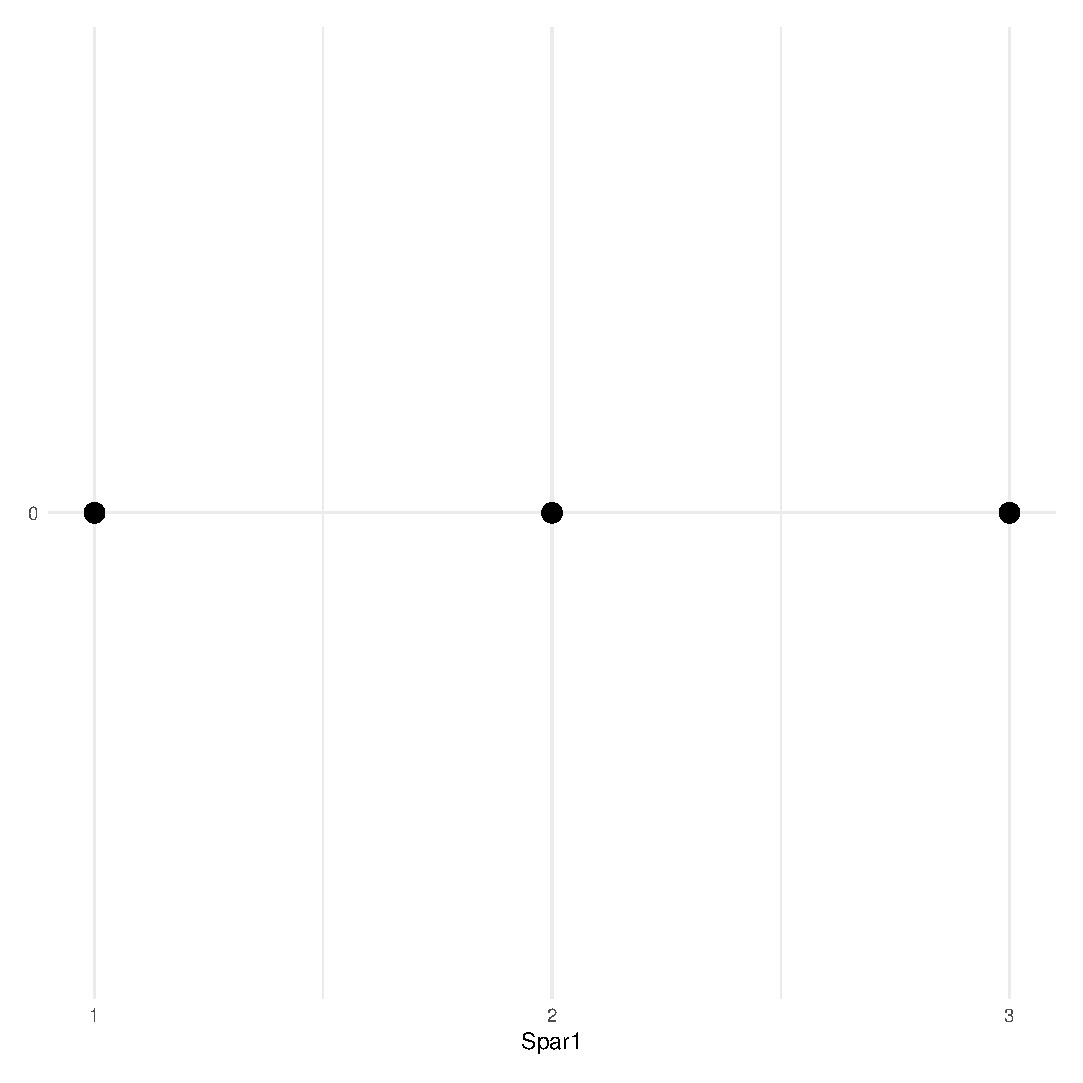
\includegraphics[width=0.9\textwidth]{../../images/points1}
  \end{minipage} %
  \begin{minipage}{0.45\textwidth}
    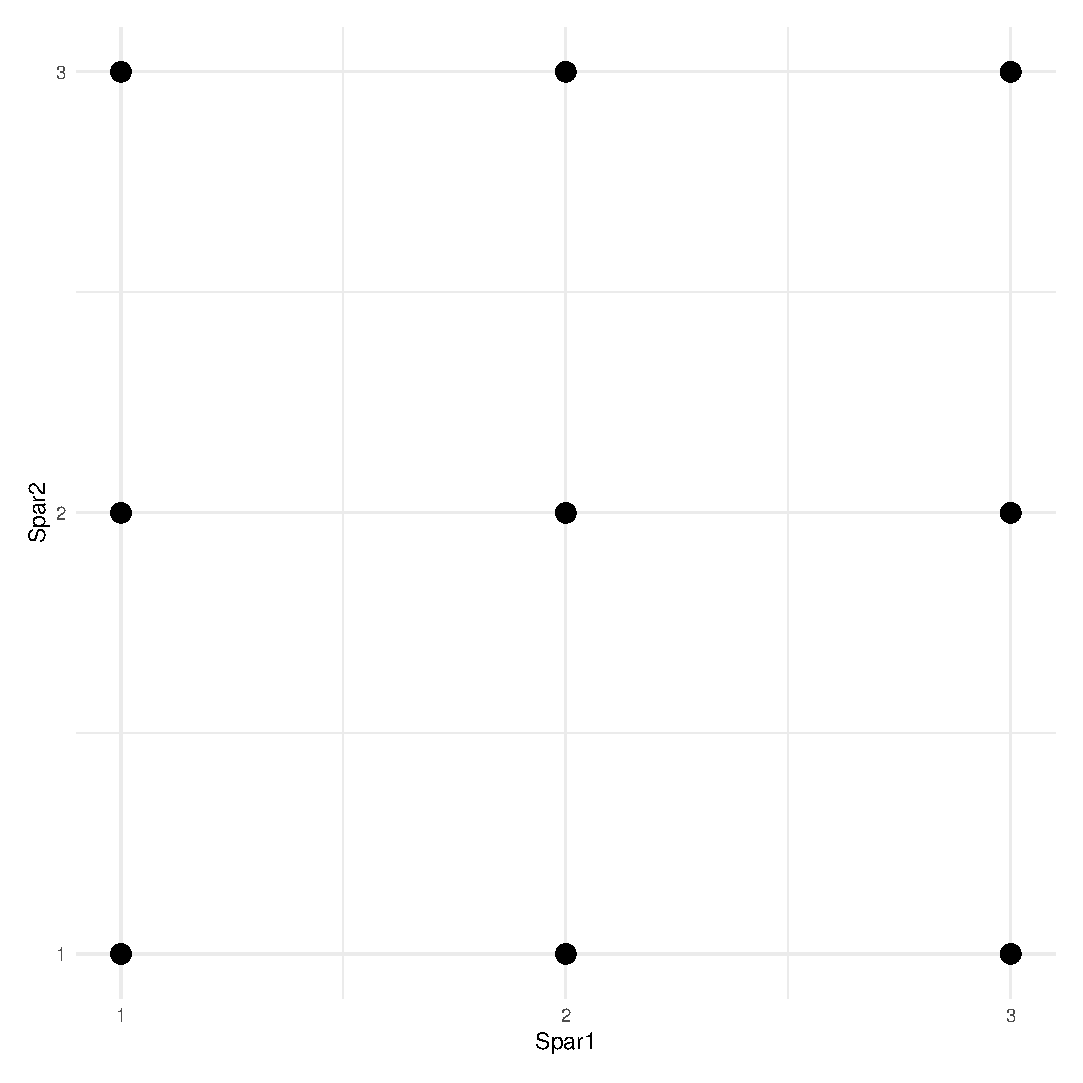
\includegraphics[width=0.9\textwidth]{../../images/points2}
  \end{minipage}
  \caption{Visual depiction of samples for $d=1$ and $d=2$.}
  \label{fig:samples}
\end{figure}

\emph{Exponential} scaling is bad, but some of the badness can be lost in
abstraction. If the one-dimensional case took $10$ seconds to execute, Table
\ref{tab:exponential} give execution times for some values of $d$. Note that by
$d=20$, the total execution time for our `simple' parameter study is already 240
times the age of the universe. Clearly, this is quite bad.

\begin{table}[!ht]
  \centering
  \begin{tabular}{r|r|l}
  \hline
  Dimension & Time (sec) & Comparison\\
  \hline
  1 & $10^{1}$ & Ten seconds\\
  \hline
  5 & $10^{5}$ & One Day\\
  \hline
  10 & $10^{10}$ & Eleven generations\\
  \hline
  18 & $10^{18}$ & Age of Universe\\
  \hline
  20 & $10^{20}$ & 230 x AoU\\
  \hline
  \end{tabular}
  \caption{Example execution times for example parameter study. Punchline exponential
    scaling is \emph{very, very bad}.}
  \label{tab:exponential}
\end{table}

This exponential scaling is one manifestation of \emph{the curse of
  dimensionality}.

\section{Curse of Dimensionality}
% --------------------------------------------------
The \textbf{curse of dimensionality}\footnote{Coined by Richard Bellman in the
  context of `exhaustive optimization'.} is the general phenomena of cost
scaling exponentially with dimension. This is actually a somewhat \emph{vague}
term, as dimensionality manifests differently across
contexts.\cite{donoho2000high} Some (academic) examples include:

\bigskip\noindent\underline{Integration:} Employing a tensor quadrature grid (as
visualized in Fig. \ref{fig:samples}) for quadrature directly leads to
exponential cost.

\bigskip\noindent\underline{Sampling:} Sampling according to a tensor design
leads to exponential cost. Note, however, that the Monte Carlo algorithm
(sampling from a density to approximate expectations) is \emph{not} cursed by
dimensionality, as Monte Carlo is dimension
independent.\cite{owen2013montecarlo}

\bigskip\noindent\underline{Machine Learning:} (Requirement of large data)

\bigskip\noindent\underline{Inference:}

\bigskip\noindent\underline{Distance:}

\bigskip\noindent\underline{Big Data:} In 2000, David Donoho gave a talk on the
curse of dimensionality as it relates to data analysis.\cite{donoho2000high}
He noted that in industry,

\begin{quote}
  The trend today is towards more observations \emph{but even more so},
  \textcolor{palered}{to radically larger numbers of variables} – voracious,
  automatic, systematic collection of hyper-informative detail about each
  observed instance.\footnote{Emphasis mine}
\end{quote}

Statisticians usually consider data in terms of a matrix; with rows representing
$n$ observations, and columns representing $d$ variables. Dimensionality is thus
`one-half' of the bigness of data.

Hopefully one of the contexts above is relevant to you. Assuming this is the
case, then dimensionality is \emph{your} problem! We've seen one way
dimensionality affects a particular context (tensor-product sampling designs),
but why does dimensionality affect all these \emph{different} contexts? To build
some intuition, let's take a look at some properties of high-dimensional
geometry.

\subsection{High-Dimensional Geometry}
% -------------------------
Why is dimensionality so challenging? Here we talk about a few properties of
high-dimensional geometry. The intent is to (1) underscore that high-dimensional
spaces have `surprising' behavior, and (2) build some intuition for
dimensionality beyond the fact that `it is challenging'.

\bigskip\noindent\underline{Fact 1:} The hypersphere has vanishing interior.

\bigskip


\begin{equation*} \begin{aligned}
    HV &= \int\cdots\int r^{d-1}\,
         T(\varphi_{1},\dots,\varphi_{d-1})\,
         dr d\varphi_{1}\cdots d\varphi_{d-1}
\end{aligned} \end{equation*}

\begin{figure}[!ht]
  \centering
  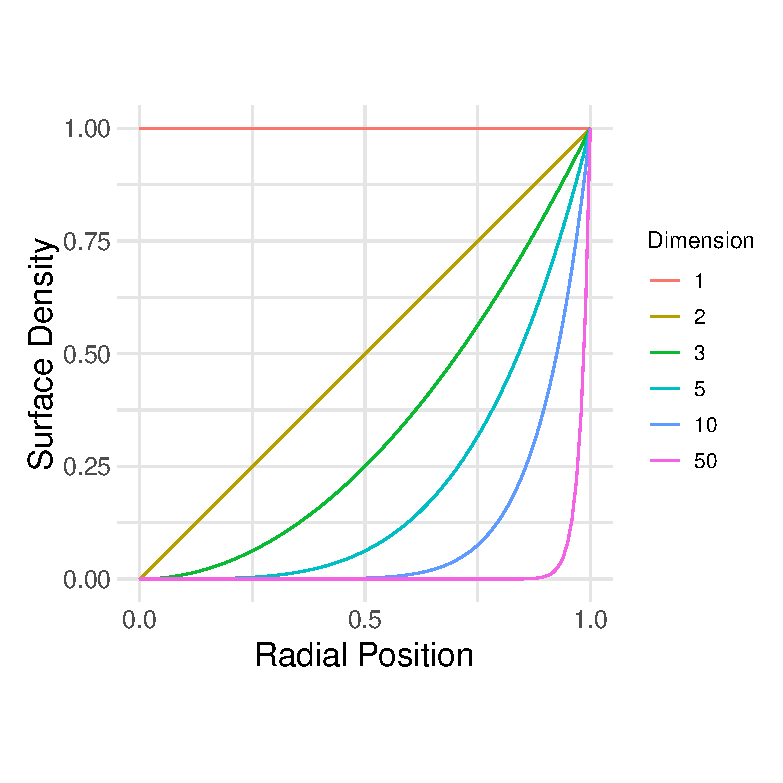
\includegraphics[width=0.65\textwidth]{../../images/surface_density}
  \caption{Radius-dependent portion of the integrant for a hypersphere volume
    calculation. Note that for higher dimensions, nearly all of the integrand is
    concentrated near the edge of $r=1$. This demonstrates that the hypersphere
    is empty -- that all of its volume is concentrated at its edge.}
  \label{fig:hypervolume}
\end{figure}

Practically, this means that if we sample uniformly from a hypersphere, then in
high dimensions, we will surely `miss' the interior. If our intent was to
understand the relation between input and response, then this is a region of a
function's input that we will not learn about. Depending on the context, this
may (or may not!) be an issue.

\clearpage
\bigskip\noindent\underline{Fact 2:} All the volume in a hypersphere is near
\emph{the} equator.

\bigskip
Upfront, this is a bit of a wordgame; there are actually \emph{many} equators on
any sphere. On Earth, we define a single equator, but one can actually think of
an infinite family of equators, each enclosed by a great circle (Fig.
\ref{fig:great-circle}). These equators are formed by intersecting a
3-dimensional sphere (a `3-sphere') with a 2-dimensional plane that passes
through the sphere's origin, forming a 2-dimensional object. Since there are
infinitely many such planes, there are infinitely many equators.

\begin{figure}[!ht]
  \centering
  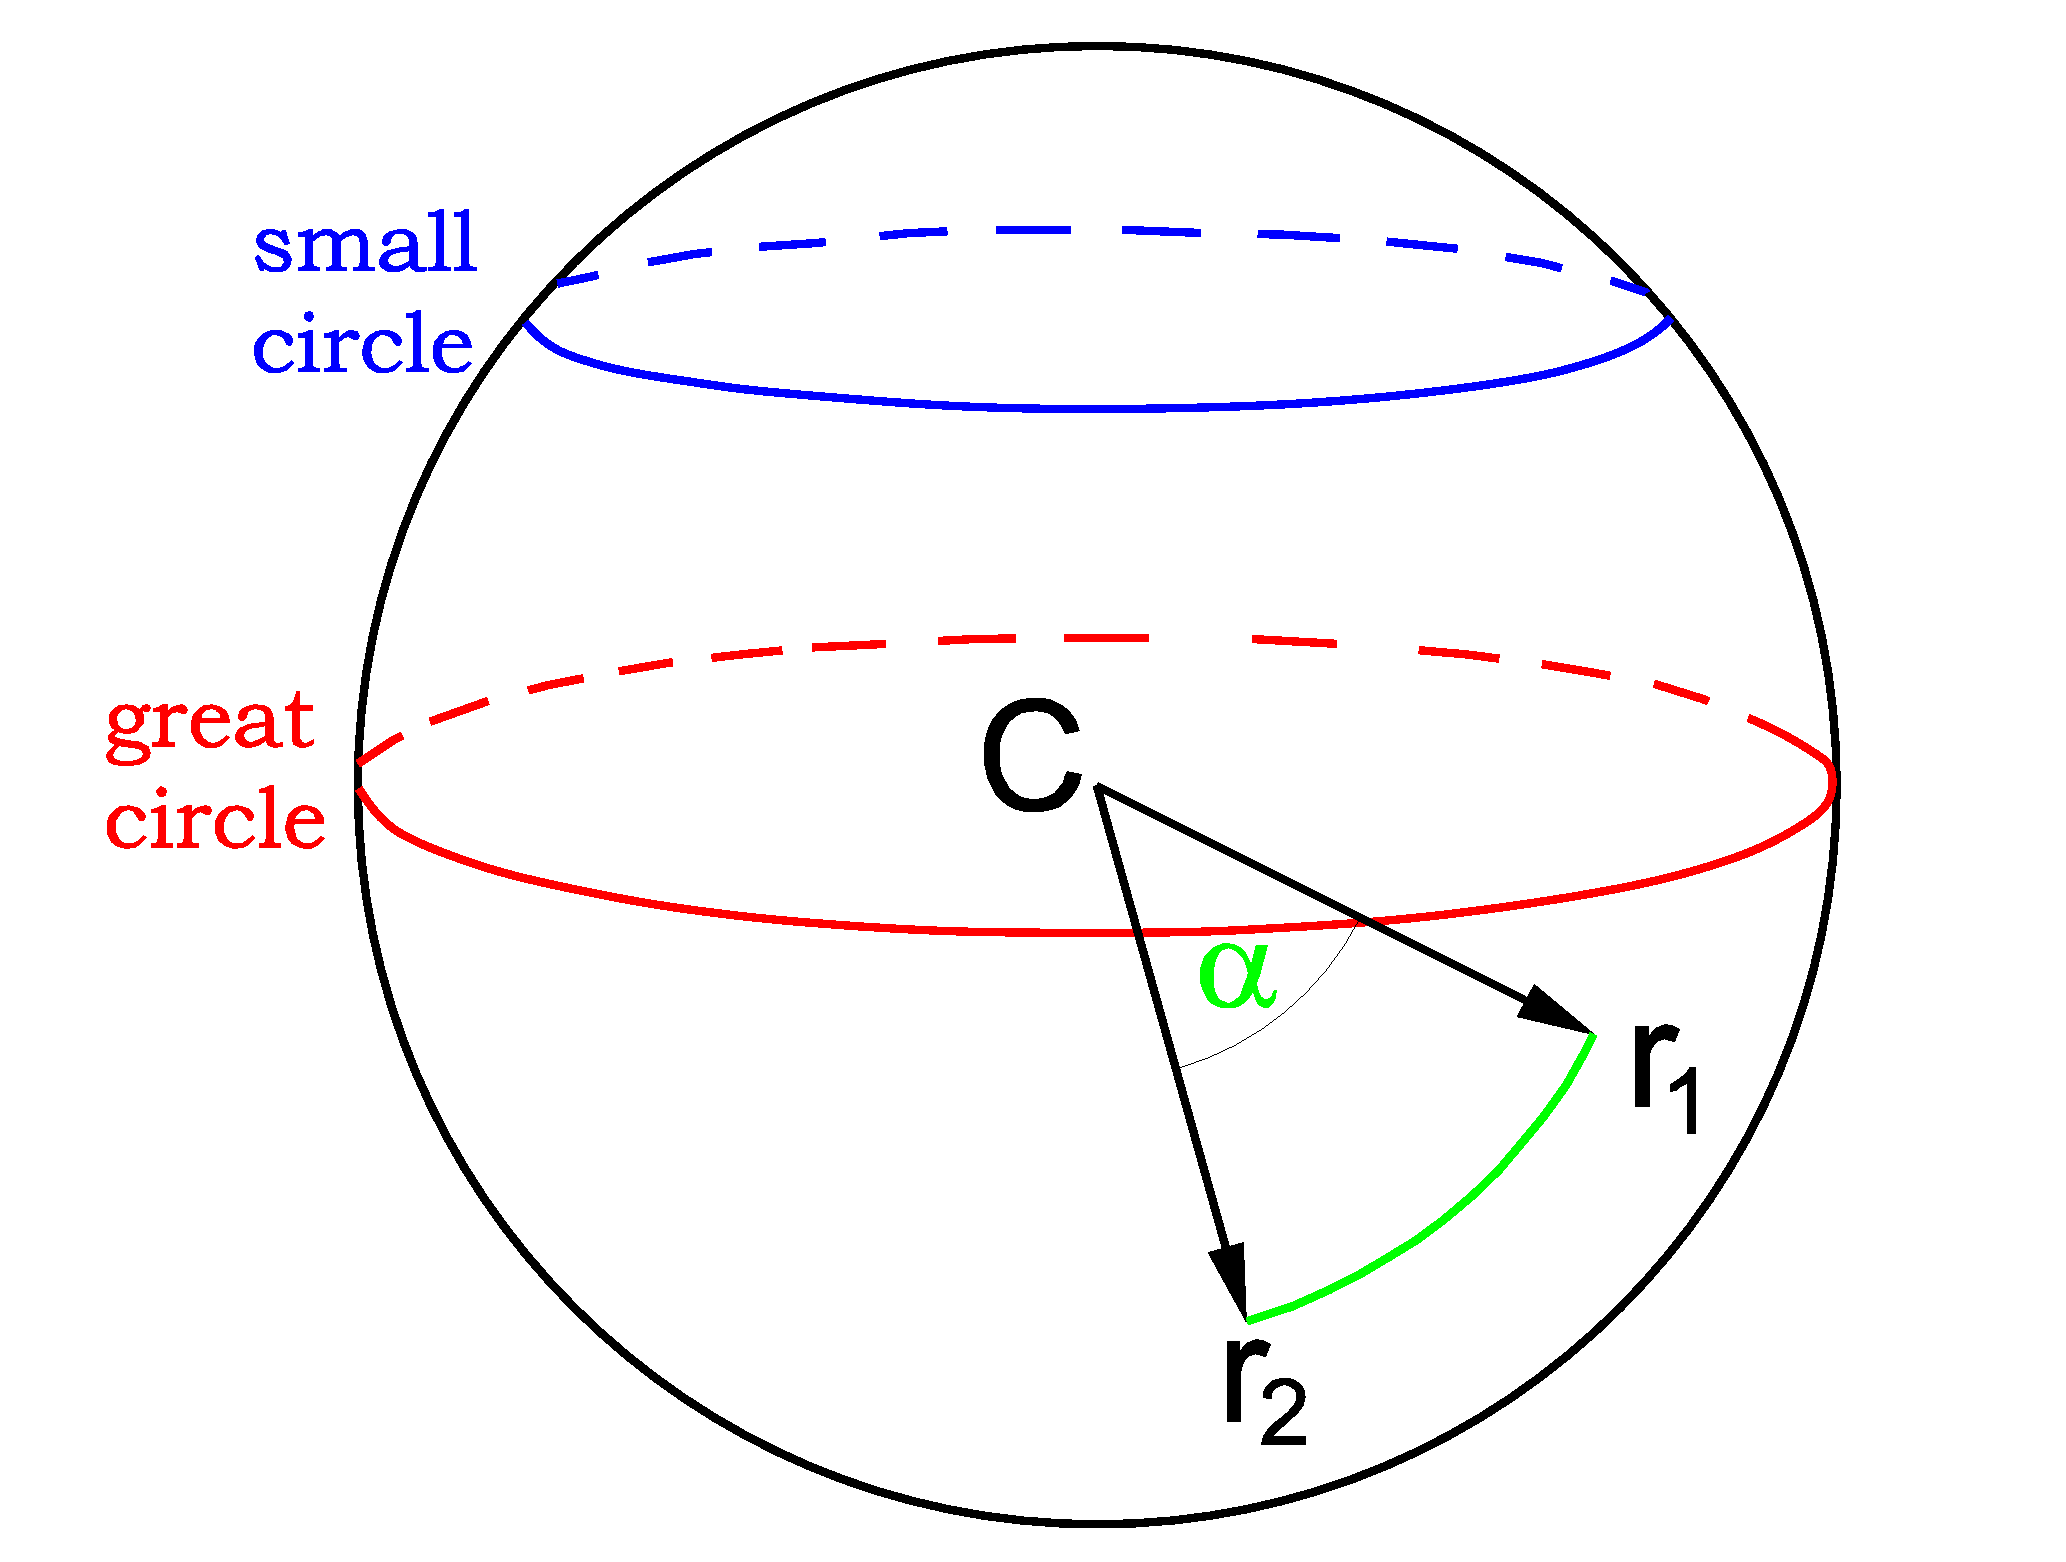
\includegraphics[width=0.65\textwidth]{../../images/great_circle}
  \caption{Cartoon depicting the boundary of a great circle for a 3-sphere. The
    red curve depicts a great circle; which encloses an equator. Thus, for the
    3-sphere, an equator is a 2-dimensional object. In higher dimensions $d$,
    the analog of an equator is a $d-1$-dimensional object. From Wikimedia
    Commons, CC P.wormer.}
  \label{fig:great-circle}
\end{figure}

In higher dimensions $d$, an equator is always a $d-1$-dimensional object. Thus,
as $d$ grows, an equator neglects proportionally less with regard to the full
dimensionality of the space. Thus, if we were to sample points uniform randomly
from within the $d$-dimensional sphere, this `neglected' dimension would
contribute less in higher dimensions. The result is that the volume -- which can
be linked to the uniform density in the hypersphere -- concentrates towards
\emph{any} chosen equator. We can see this by picking an arbitrary equator,
sampling at random, and computing the histogram of angles formed by the vector
between drawn points, the origin, and the chosen equator. Figure
\ref{fig:equator} shows results from this computer experiment: The realized
angles concentrate towards zero as $d$ increases.

\begin{figure}[!ht]
  \centering
  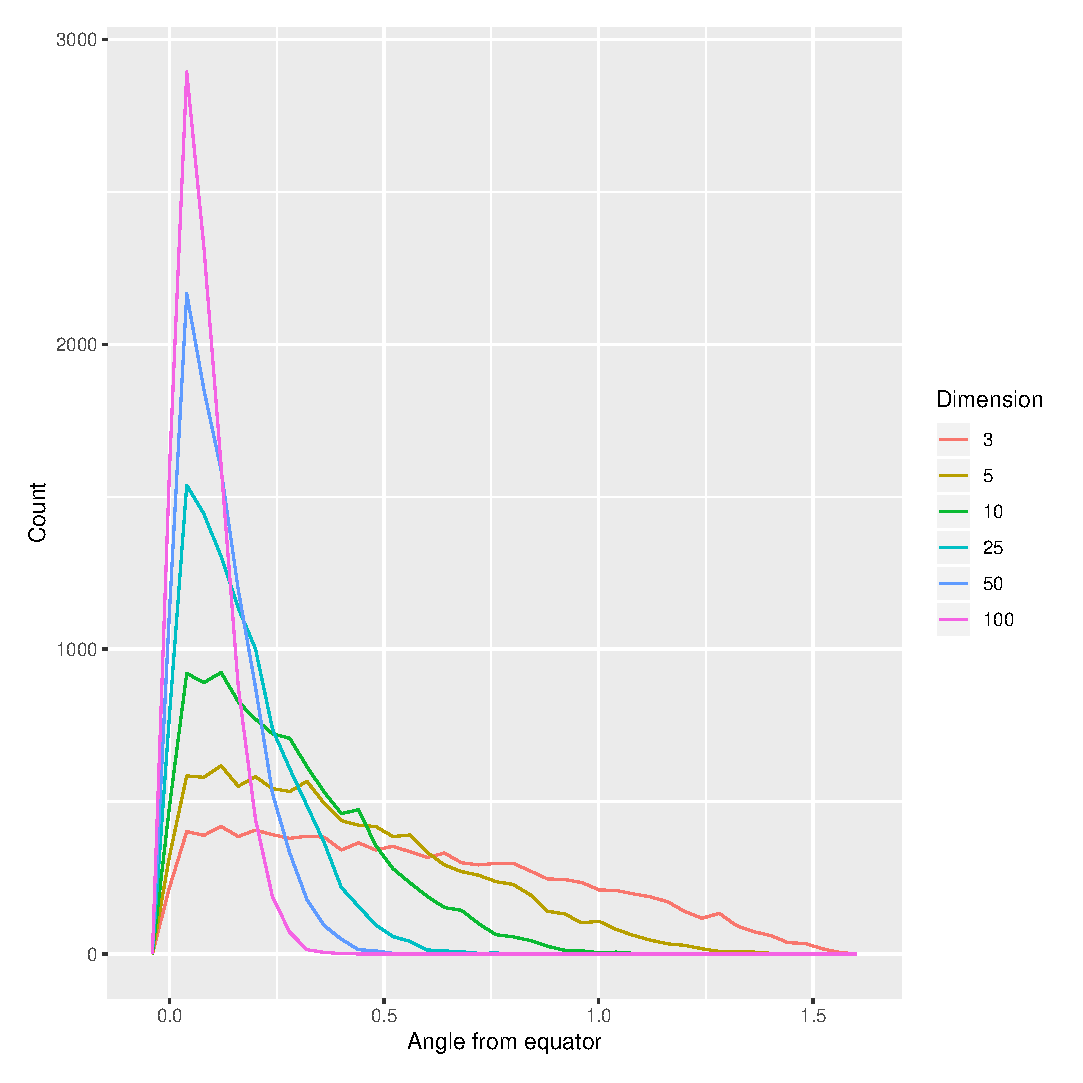
\includegraphics[width=0.65\textwidth]{../../images/equator}
  \caption{Realized angles away from a chosen equator for a $d$ dimensional
    hypersphere, estimated as empirical densities. This illustrates that, as
    $d\to\infty$, most points in the hypersphere (thus the volume) are
    concentrated near an equator.}
  \label{fig:equator}
\end{figure}

Similar to above, in high dimensions we will `miss' some \emph{directions} when
sampling uniformly from the hypersphere.

\clearpage
\bigskip\noindent\underline{Fact 3:} Random projections preserve pairwise
distances.

\bigskip
First, we'll illustrate this fact with an example, then describe the theorem
that backs it up. I use some gene expression data from the UC Irvine machine
learning databse\cite{blake1998uci} for this example.\footnote{The specific data
  source is not terribly important here; the point is that the data are not
  `cooked' for demonstration purposes.} The data are loaded into the variable
\lstinline{mat_data}; the data have dimensions

\begin{lstlisting}
## Gene data from UCI
dim(mat_data)
#       Observations,  Dimensions
> [1]   801,           20531
\end{lstlisting}

We select a random projection of dimensionality \lstinline{k} via some
mysterious, to-be-described procedure, based on a user-selected error tolerance
\lstinline{eps}.

\begin{lstlisting}
## Make reproducible
set.seed(101)
## Calculate dimension
C <- 1                             # Over-samping factor
n <- dim(mat_data)[1]              # Observations
d <- dim(mat_data)[2]              # Dimensionality

k <- C * ceiling(log(n) / eps ^ 2) # J-L dimension
k
> 1338 (6.5% of 20531)
\end{lstlisting}

This mysterious procedure has suggested a projection of dimensionality $1338$,
just $6.5\%$ of $20531$.

A bonus fact is that, in high dimensions, random vectors drawn from an isotonic
gaussian\footnote{A gaussian possessing a diagonal covariance matrix} will
essentially be orthogonal.\cite{ailon2009fast} We can use this fact to easily
construct a random projection of the desired size.

\begin{lstlisting}
## Random `projection`
P <-
  rnorm(d * k, sd = 1 / d) %>%
  matrix(nrow = d, ncol = k)
## Project the data
mat_proj <-
  mat_data %*% P
\end{lstlisting}

When we project to a smaller dimensionality, we tend to decrease the average
distance between points. To have any hope of preserving pairwise distances, we'd
better account for this fact.

\begin{lstlisting}
## Match the original average distance; Subsample for speed
Ind <- sample(x = 1:n, size = 500)

D_sub_orig <-
  mat_data[Ind, ] %>%
  dist()

D_sub_fix <-
  mat_proj[Ind, ] %>%
  dist()

factor <-
  mean(D_sub_orig, na.rm = TRUE) / mean(D_sub_fix, na.rm = TRUE)

mat_proj <-
  mat_proj * factor
\end{lstlisting}

The claim is that the projected data \lstinline{mat_proj} possesses the same
pairwise distances $\|\vu-\vv\|$ as \lstinline{mat_data}, to within the chosen
tolerance \lstinline{eps}; let's check if that is the case.

\begin{lstlisting}
## Re-compute distances with proper scaling
Ind <- sample(x = 1:n, size = 500) # New draw

D_sub_orig <-
  mat_data[Ind, ] %>%
  dist()

D_sub_proj <-
  mat_proj[Ind, ] %>%
  dist()

## Compute quantiles of discrepancy
R_diff <- (D_sub_proj - D_sub_orig) / D_sub_orig
qt <- quantile(R_diff)
## qt
sprintf(
  "%5.3f%% %5.3f%% %5.3f%% %5.3f%% %5.3f%%",
  qt[1] * 100,
  qt[2] * 100,
  qt[3] * 100,
  qt[4] * 100,
  qt[5] * 100
)
>      0%     25%    50%    75%   100%
> -7.784% -1.193% 0.082% 1.344% 8.139%
\end{lstlisting}

In this case, the realized distortion is indeed within $\pm10\%$. This is a bit
mysterious -- by \emph{randomly} throwing out information, we were able to
preserve a great deal of structure in the data. The
\textbf{Johnson-Lindenstrauss lemma} (J-L) shows that this is no accident, but
rather a general property of high-dimensional spaces.

\bigskip
\underline{Lemma:} (Johnson-Lindenstrauss) For any $0<\epsilon<1$ and
$n\in\mathbb{Z}_{>0}$, let $k\in\mathbb{Z}_{>0}$ such that

\begin{equation} \label{eq:jl-bound}
  k \geq C \frac{\log(n)}{\epsilon^2},
\end{equation}

\noindent then for all sets of points $V\subset\R{d}$, there is a projection
$P_k:\R{d}\to\R{k}$ with $\alpha\in\R{}_{>0}$ such that, for all $u,v\in V$, we
have

\begin{equation} \label{eq:jl-distance}
  (1 - \epsilon)\|\vu - \vv\|^2 \leq \alpha\|P_k(\vu) - P_k(\vv)\|^2 \leq %
  (1 + \epsilon)\|\vu - \vv\|^2.
\end{equation}

\noindent Further, this projection can be found in polynomial time.

\bigskip
Numerous proofs of this statement\footnote{note that I've modified the statement
  above to emphasize certain elements, in the interest of aiding explanation.
  The `true' J-L lemma is stated slightly differently; I've made $\alpha$
  explicit in the statement above} exist, for an example see Dasgupta and
Gupta.\cite{dasgupta2003elementary}

Let's first try to understand the statement above. \Cref{eq:jl-distance} is a
statement about pairwise distances $\|\vu-\vv\|$ and their projected versions
$\|P_k(\vu) - P_k(\vv)\|$. J-L states that \emph{all} points in a given (data)
set satisfy this condition. Precisely, the projected pairwise distances can only
be distorted at most by a factor of $(1\pm\epsilon)$.

Note that the projected pairwise distances are multiplied by a positive value
$\alpha$. This is because projections reduce the \emph{average} distance between
points, as illustrated in Figure \ref{fig:jl-avg-distance}. If we want any hope
of matching pairwise distances, we have to account for this fact. I do this very
simply in the code above by computing $\alpha$ from the ratio of average
distances between the original and projected data -- we then restore by
multiplying by alpha.

\begin{figure}[!ht]
  \centering
  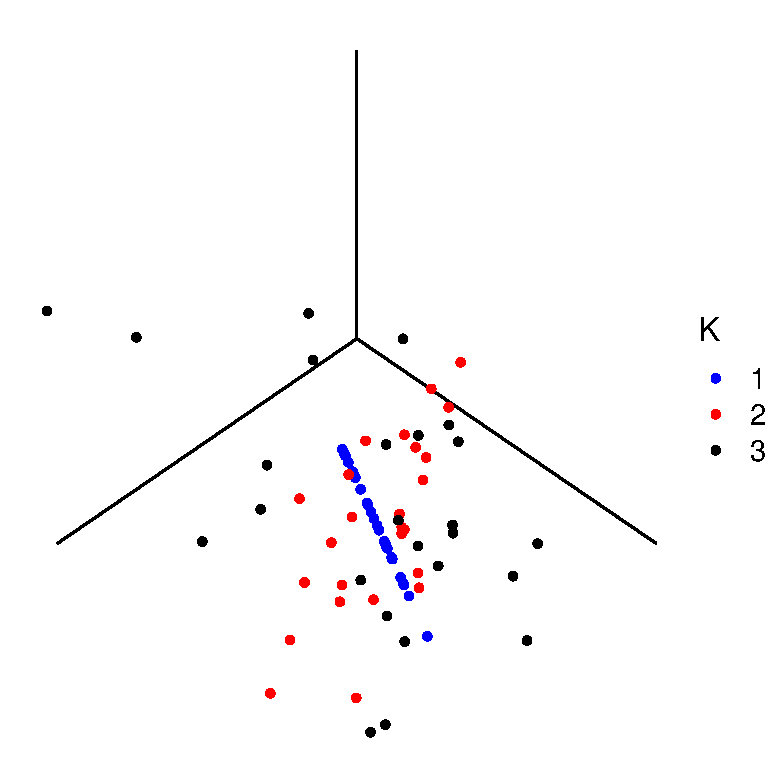
\includegraphics[width=0.65\textwidth]{../../images/dim_proj1}
  \caption{Example points in 3d space, projected to lower dimensions. Note the
    average distance between points is reduced with successively smaller
    projections.}
  \label{fig:jl-avg-distance}
\end{figure}

\Cref{eq:jl-bound} provides a target dimensionality based on provided
quantities. Provided the number of observations $n$ and desired error tolerance
$\epsilon$, J-L suggests a minimum projection dimension $k$. Note that
\emph{dimensionality is absent} from this bound. The original dimensionality $d$
can be arbitrarily large; given the same $n$ and $\epsilon$, the bound on
projection dimension will be the same.

This dimensionality $k$ is something we'll refer to -- in a somewhat
\emph{vague} sense -- as \emph{intrinsic dimensionality}. Within a space of
dimension $d$, there is low-dimensional structure of size $k$ (the mapping
$\alpha P_k(\cdot)$) that preserves information of interest, here pairwise
distances. This points forward to a general strategy for lifting the curse of
dimensionality -- if we can identify low-dimensional that preserves the
properties we care about, then we can reduce the effective dimensionality from
$d$ to $k$, and (potentially) render tractable the problems we want to solve.
This is the idea behind \emph{dimension reduction}.

\section{Dimension Reduction}
% --------------------------------------------------

\textbf{Dimension reduction} is the general strategy of identifying some form of
low-dimensional structure within a problem. Since there are many different
problem settings and objectives -- thus many \emph{kinds} of structure -- we
introduce a simple taxonomy to help distinguish different flavors of dimension
reduction.

\subsection{A Taxonomy}
% -------------------------
We will discuss three flavors of dimension reduction, broadly categorized by the
interpretation of $\R{d}$. Note that many of the techniques we will introduce
are applied across different contexts -- the mathematics does not appreciably
change in these different settings. However, the \emph{interpretation} of
mathematics changes across settings; if we seek to understand how the math
applies to our particular setting -- and if we seek to understand work by other
researchers in different fields -- then this difference in interpretation is
meaningful.

For instance, the singular value decomposition (SVD) shows up under different
names in different communities: the Karhunen-Loeve expansion (KLE), the proper
orthogonal decomposition (POD), principal component analysis (PCA), etc.
Mathematically, there is little difference between these ideas. However, a
person using the term KLE will generally be thinking of a different kind of
problem than someone speaking of PCA. Further, different properties of the SVD
are relevant in these different contexts. Both the communication aims and
technical details are conveyed by the different terminology.

We will describe the taxonomy of different settings, then focus on the
\emph{input-space} setting to give a bit more detail.

\bigskip\noindent A \underline{generic-space} is $\R{d}$ with no special
assumptions. Techniques like the Johnson-Lindenstrauss lemma and principal
component analysis\cite{fodor2002survey} are used in this context.

\bigskip\noindent An \underline{output-space} is $\R{d}$ understood as the
output of some (dynamical) system; the $d$ entries of a vector from $\R{d}$
could represent a time-varying signal (e.g. a speech sample), the pointwise
entries of some field (e.g. a mean channel-flow field), or some combination
(e.g. a time-varying flow field). The techniques of compressed sensing
(CS)\cite{candes2008introduction} and the proper orthogonal
decomposition\cite{lumley2007} are often used in this context.

\bigskip\noindent An \underline{input-space} is $\R{d}$ understood as the input
space to some function $f(\vx)$. Compressed sensing is also used in this
context,\cite{tang2014subsampled} but other approaches are a bit more common. We
will discuss these below, under additional broad categorizations.

\subsection{Input-space: Running Example}
% -------------------------
To explore input-space dimension reduction techniques, we first introduce the
simple illustrative problem of rough pipe flow, like that originally studied by
Osborne Reynolds.\cite{reynolds1883}

\begin{figure}[!ht]
  \centering
  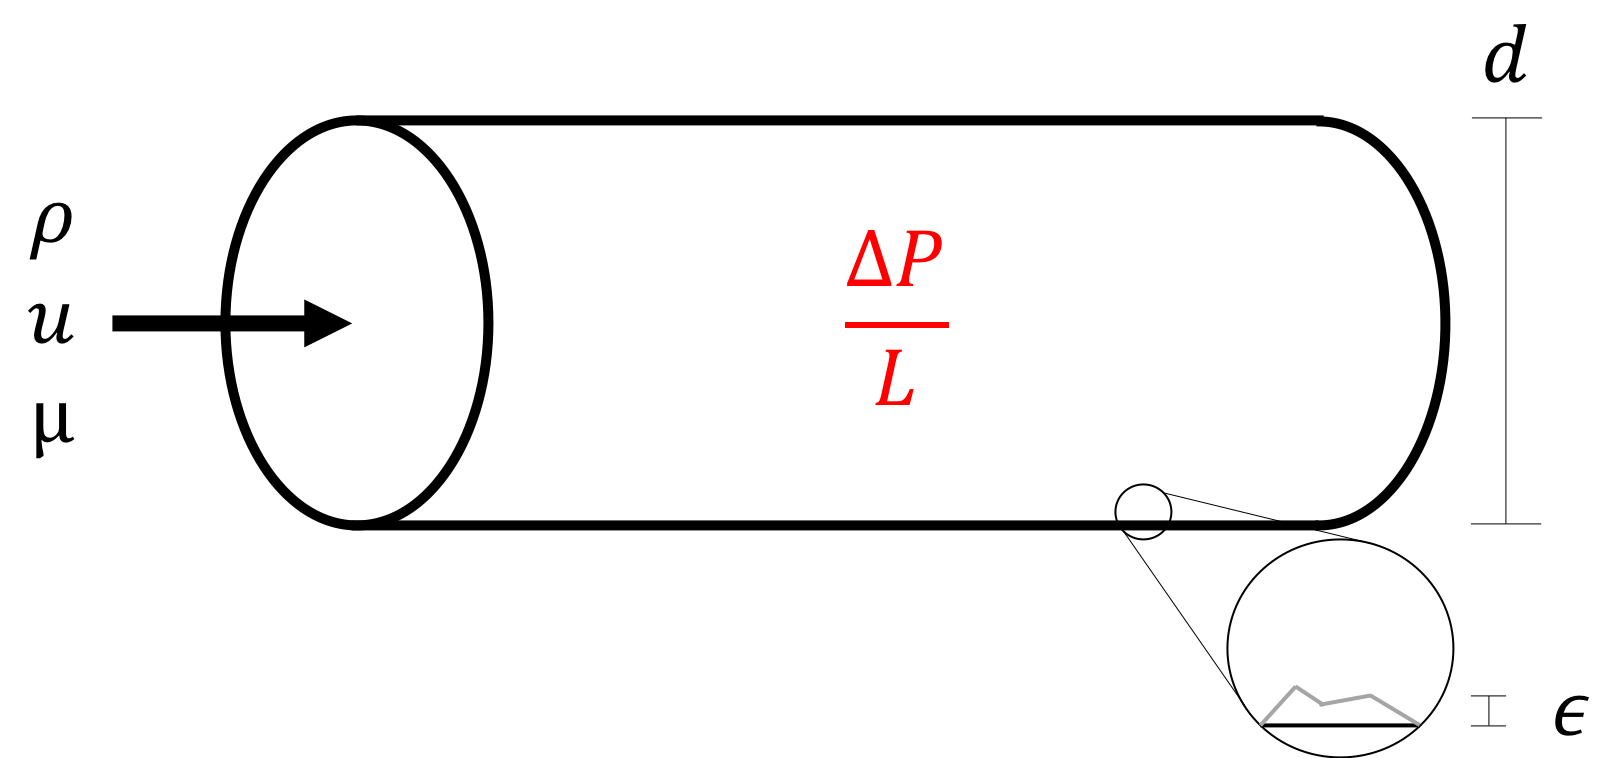
\includegraphics[width=0.65\textwidth]{../../images/pipe_diagram}
  \caption{Schematic for example pipe flow problem. A viscous fluid is pumped
    through a rough pipe. Our output quantity of interest is the (normalized)
    pressure loss -- a measure of the effort required to pump the fluid. The
    inputs are the fluid properties and pipe geometry.}
  \label{fig:pipe_diagram}
\end{figure}

\subsection{Subset Reduction}
% -------------------------
\textbf{Morris screening}

\textbf{Sobol' indices}

\subsection{Subspace Reduction}
% -------------------------
\textbf{Principal component analysis}

We can think of the \textbf{active subspace} as an object arising from a PCA on
gradient data; in fact, an early formulation of the active subspace was exactly
posed as such.\cite{russi2010uncertainty}

\section{Intrinsic Dimensionality}
% --------------------------------------------------

\bibliographystyle{plain}
\bibliography{bibtex_database}

\end{document}
